\documentclass{article}
\usepackage[utf8]{inputenc}
\usepackage{indentfirst}
\usepackage{titling}
\usepackage{geometry}
\usepackage{graphicx}
\graphicspath{ {./Images/} }
\usepackage[shortlabels]{enumitem}
\usepackage{fancyhdr}
\usepackage{ulem}
\usepackage[dvipsnames]{xcolor}
\usepackage{amssymb}
\usepackage{listings}
\usepackage{color}

\definecolor{dkgreen}{rgb}{0,0.6,0}
\definecolor{gray}{rgb}{0.5,0.5,0.5}
\definecolor{mauve}{rgb}{0.58,0,0.82}

\lstset{frame=tb,
  language=Java,
  aboveskip=3mm,
  belowskip=3mm,
  showstringspaces=false,
  columns=flexible,
  basicstyle={\small\ttfamily},
  numbers=none,
  numberstyle=\tiny\color{gray},
  keywordstyle=\color{blue},
  commentstyle=\color{dkgreen},
  stringstyle=\color{mauve},
  breaklines=true,
  breakatwhitespace=true,
  tabsize=3
}

\def\ojoin{\setbox0=\hbox{$\bowtie$}%
  \rule[-.02ex]{.25em}{.4pt}\llap{\rule[\ht0]{.25em}{.4pt}}}
\def\leftouterjoin{\mathbin{\ojoin\mkern-5.8mu\bowtie}}
\def\rightouterjoin{\mathbin{\bowtie\mkern-5.8mu\ojoin}}
\def\fullouterjoin{\mathbin{\ojoin\mkern-5.8mu\bowtie\mkern-5.8mu\ojoin}}

\renewcommand\maketitlehooka{\null\mbox{}\vfill} %para centralizar verticalmente
\renewcommand\maketitlehookd{\vfill\null}
\pagestyle{fancy}
\fancyhf{}
\rfoot{\thepage}
\lfoot{ 
\includegraphics[scale=0.01]{UA.jpg} José Mendes 107188 LEI}
\geometry{
  a4paper,
  headheight=4cm,
  top=5.5cm,
  bottom=4.5cm,
  footskip=4cm
}


\title{Complementos de Bases de Dados}
\author{José Mendes 107188}
\date{2023}

\begin{document}


\begin{titlepage}
    \maketitle
    \begin{center}
        
\includegraphics[scale=0.4]{UA.png}
    \end{center}
    \thispagestyle{empty} %remove o count da pagina
\end{titlepage}

\pagebreak
%depois por um index aqui

\section{Evolução dos Sistemas de Base de Dados}

\begin{flushleft}
    \textbf{Sistemas de Dados -} Cada vez mais as aplicações de hoje em dia
    são Data-Intensive, em vez de Compute-Intensive. 

    Para Data-Intensive, o poder bruto da CPU deixa de ser um fator limitante
    quando comparado com a \textbf{quantidade}, \textbf{complexidade} e \textbf{velocidade de atualização} dos dados.

    \vspace{3mm}

    De forma a otimizar a sua performance, um sistema de dados tipicamente oferece as seguintes
    funcionalidades:
    \begin{enumerate}
      \item \textbf{Bases de Dados -} armazenam os dados para utilização futura;
      \item \textbf{Caches -} guardam os resultados de operações dispendiosas, de forma a tornar a leitura mais rápida;
      \item \textbf{Search Indexes -} permitem aos utilizadores procurarem por palavras-chave ou filtrar os dados;
      \item \textbf{Message Queues -} permitem a comunicação assíncrona entre processos;
      \item \textbf{Stream Processing -} permite o processamento de dados em tempo real;
      \item \textbf{Batch Processing -} permite o processamento de dados acumulados, periodicamente;
    \end{enumerate}

    \textcolor{Blue}{Exemplo:}
    Um exemplo de \textbf{stream processing} ocorre na banca. Sempre que é realizada uma transação, os dados da mesma são
  imediatamente processados de forma a que o saldo esteja sempre atualizado.


  O \textbf{batch processing} é visível na faturação dos serviços pós-pagos pelas operadoras de telecomunicações. No final de
  cada mês, é feita uma consulta às suas bases de dados de forma a identificar todos os consumos do cliente, que são
  somados e depois gerada a fatura.


  No \textbf{stream} os dados são processados antes de armazenados, enquanto que no \textbf{batch} são processados depois de
  armazenados.

  \vspace{3mm}

  Cada vez mais as aplicações requerem um \textbf{maior wide-range de requisitos}. Muitas das vezes,
  \uline{uma única ferramenta já não consegue satisfazer todas as necessidades de \textbf{data processing} e \textbf{storage}}.

  \vspace{2mm}

  Em vez disso, o \uline{trabalho é partido em tasks que possam ser realizadas de forma eficiente
  por uma única ferramenta}. As ferramentas individuais utilizadas são depois juntas utilizando
  código de aplicação.

  \vspace{2mm}

  \textcolor{Blue}{Exemplo:} Podemos ter uma aplicação que utiliza uma Catching Layer (\textbf{memcached}), um Full-Text Search (\textbf{Elasticsearch})
  e uma Base de Dados principal separada (\textbf{MySQL}).
\end{flushleft}

\begin{center}
  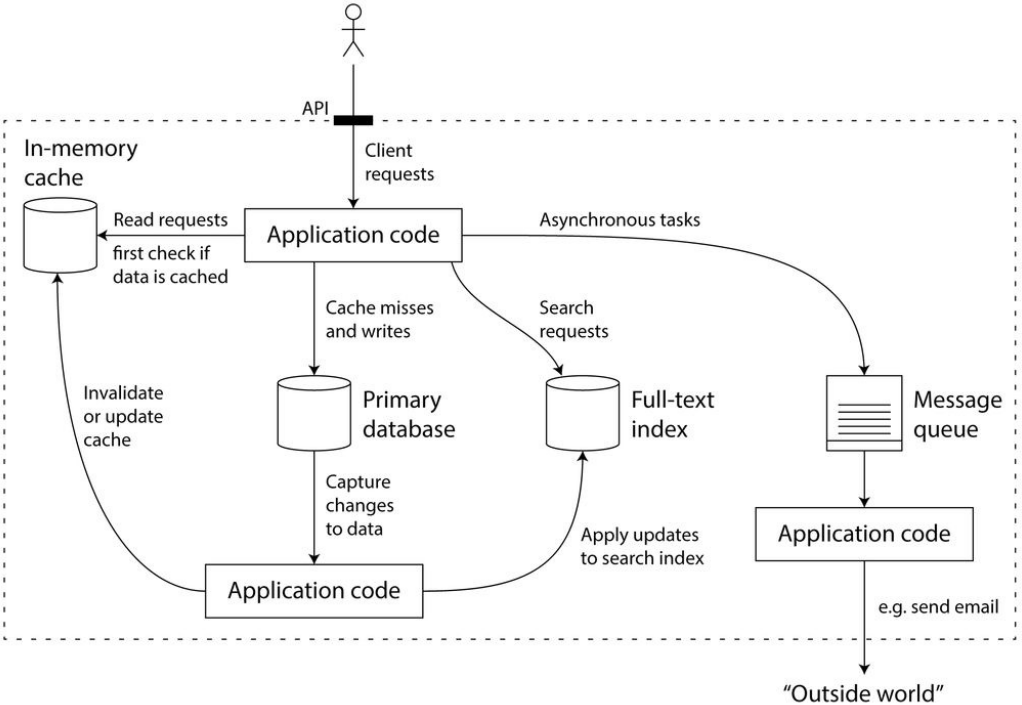
\includegraphics[scale=0.3]{1.png}
\end{center}

\subsection{Desafios que os Sistemas de Dados enfrentam}

\begin{flushleft}
  \item Como garantir que todos os dados se mantêm corretos e consistentes, mesmo quando, internamente, ocorreu algum erro? (ex: persistência de dados)
  \item Como fornecer boa performance para os clientes, mesmo quando partes do sistema estão degredadas?
  \item Como escalar o sistema para ser capaz de aguentar uma load intensiva de trabalho?
  \item Qual a aparência de uma boa API para o serviço?
\end{flushleft}

\subsection{Alguns Requisitos}

\begin{flushleft}
  \item \textbf{Fiabilidade -} O Sistema deve continuar a funcionar corretamente em caso de adversidades (ex: falhas de hardware, software ou mesmo humanas).
  \item \textbf{Escalabilidade -} O Sistema deve ser capaz de responder ao crescimento seja do volume de dados, do tráfego, ou mesmo da complexidade.
  \item \textbf{Manutenibilidade -} Deve ser possível que o Sistema sofra alterações ao longo do tempo por várias pessoas diferentes de forma produtiva.
\end{flushleft}

\pagebreak

\subsection{Bases de Dados}

\begin{flushleft}
  São definidas como um \uline{conjunto de dados relacionados entre si e a sua organização}.
  \vspace{2mm}
  Dividem-se em vários tipos, sendo atualmente os mais comuns: \textbf{Relacionais}, seguidas por
  \textbf{Documentais}, \textbf{Motores de busca}, \textbf{Chave-Valor}, entre outras. 
  \vspace{2mm}
  O controlo às bases de dados é realizado por \textbf{Sistemas de Gestão de Base de Dados} (\textbf{SGBD}
  ou DBMS em inglês). Estes fornecem funções que permitem a manipulação de grandes
  quantidades de informação.
\end{flushleft}

\section{NoSQL Databases - Key-Value Databases}

\begin{flushleft}
  \begin{enumerate}
    \item É o mais simples dos tipos NoSQL;
    \subitem Consiste apenas em chaves únicas e a um "bucket" que contêm qualquer tipo de dados que se pretenda;
    \item Pares chave-valor:
    \subitem \textbf{Chave}: (id, identificador, chave primária) Normalmente é uma String;
    \subitem \textbf{Valor}: Pode ser qualquer tipo de dados, texto, estrutura, imagem \dots;
    \item O conteúdo do valor ("bucket") pode ser, literalmente, qualquer coisa (mais comum é não estruturado ou semi-estruturado);
    \item Os "buckets" podem armazenar entradas pesadas, incluindo BLOBs (Basic Large Objects);
    \item Row based systems, utilizados para eficiência;
  \end{enumerate}
\end{flushleft}

\subsection{Vantagens}

\begin{enumerate}
  \item Tolerância a falhas elevada - sempre disponível;
  \item Schemaless, logo, muito flexível. oferece uma grande escalabilidade para mudar os requisitos dos dados;
  \item Eficiente a devolver dados de um objeto, com operações de disco minimas;
  \item Muito simples, rápido e fácil de dar deploy;
  \item Ótimo para escalabilidade horizontal (muitos servidores);
  \item Não necessita de queries SQL, indexes, triggers, sp's, views, \dots;
  \item Data ingest rates muito elevadas (muitos dados a entrar);
  \subitem Favorece: escreve uma vez, lê muitas vezes;
  \item Potente no "offline reporting" com data sets muito grandes;
  \item Existem formas avançadas de KVs que apresentam capacidades de document ou column oriented stores;
\end{enumerate}

\pagebreak

\subsection{Desvantagens}

\begin{enumerate}
  \item Não é apropriado para aplicação complexas;
  \item Não é eficiente a ataualizar records em que apenas parte do "bucket" é alterado;
  \item Não é eficiente em devolver informação limitada de records específicos (ex: returning only
  records of employees making between \$40K and \$60K); 
  \item Não é apropriado para queries complexas;
  \item Com o aumento do volume de dados, manter chaves únicas pode tornar-se um problema;
  \item Geralmente precisa de ler todos os records de um "bucket" ou talvez precise de contruir índices secundários;
\end{enumerate}

\subsection{Use Cases}

\begin{enumerate}
  \item Session data, user profiles, user preferences, shopping
  carts, \dots;
  \item Criar datasets que são raramente acessados mas crescem ao logo do tempo (Caching);
  \item Onde a performance de escrite é a prioridade;
\end{enumerate}

\subsection{Quando NÃO usar}

\begin{enumerate}
  \item Quando precisamos de ter relações entre entidades;
  \item Queries requerem acesso a conteúdos da parte dos valores;
  \item Set operations que envolvem múltiplos pares chave-valor;
\end{enumerate}

\subsection{Key Management}

\begin{flushleft}
  Como devem as chaves serem produzidas?

  \item \textbf{Manualy assigned keys} - Identificadores do mundo real (ex: e-mail, login names, \dots);
  \item  \textbf{Automatically generated keys} - Auto-incremente integers ou chaves mais complexas geradas por algotitmos;
\end{flushleft}


\pagebreak

\subsection{Query Patterns}

\begin{enumerate}
  \item Basic \textbf{CRUD} operations;
  \subitem Apenas quando a chave for dada;
  \subitem O conhecimento da chave é essencial;
  \subitem Ás vezes, pode ser até dificil para uma base de dados dar uma lista com todas as chaves;

  \item \textbf{No searching by value};
  \subitem Mas pode-se instruir à base de dados como dar parse aos valores, para fazer operações;

  \item \textbf{Batch / sequential processing}
  \subitem MapReduce;
\end{enumerate}

\subsection{Outras funcionalidades}

\begin{enumerate}
  \item Expiração de  pares chave-valor;
  \item Coleções de valores (We can store not only ordinary values, but also their
  collections such as ordered lists, unordered sets etc.);
  \item Links entre pares chave-valor (podem ser usados quando se usa queries);
\end{enumerate}

\subsection{Exemplos}

\begin{enumerate}
  \item \textbf{RiakKV}
  \item \textbf{Redis}
\end{enumerate}

(Ver slides 12-40)

\section{NoSQL Databases - Document Databases}

As bases de dados de documentos são bastante eficientes em cenários \textbf{one-to-many}.
Oferecem um esquema flexível (mesmo dentro das mesmas coleções (informação heterogénia)) e melhor performance
(devido ao armazenamento da informação junto à entidade a que esta se refere) que são
manipulados através de código simples.

\begin{flushleft}
  \textbf{Nota:} A flexibilidade permite que existam objetos na mesma coleção com atributos ligeiramente diferentes, sem necessidade
  de criarmos uma tabela para cada tipo de objeto.

  A localidade pode levar à duplicação de dados entre documentos.
\end{flushleft}

Um \textbf{documento} caracteriza-se por uma \textbf{string continua} codificada em JSON, XML,
ou outro formato binário estruturado.
É self-described (atributos são claros) e apresentam uma \textbf{estrutura em árvore}. São
identificados por um \textbf{id único}.

Geralmente, para manipular, é necessário carregá-lo por completo e para guardar as
alterações reescreve-lo na totalidade.

\begin{flushleft}
  \textbf{Nota:} A localidade só se torna uma vantagem se manipularmos porções grandes do documento.
\end{flushleft}

\pagebreak

Esta topologia não aplica a modelos \textbf{many-to-many}, pois não existem
operações de \textbf{join} de documentos. Deve também ser evitada quando a estrutura
do documento é demasiado instável (sempre a mudar).

\begin{flushleft}
  \textbf{Nota:} Não é desejável demasiada granularidade entre os documentos porque se todos apresentarem características
  diferentes não são relacionáveis e assim não fará sentido estarem na mesma coleção.
\end{flushleft}

No entanto, é a ideal para logging de eventos, sistemas de gestão de conteúdos,
blogues, web analytics, aplicações e-commerce \dots
Por ser a solução para alguns, mas não para todos os problemas, as bases de dados
relacionais começaram a incluir funcionalidades documentais e vice-versa.

\subsection{Exemplos}
  \begin{enumerate}
    \item \textbf{MongoDB}
    \item \textbf{CouchDB}
    \item \textbf{Couchbase}
  \end{enumerate}
  (Ver slides 11-51)

\section{Modelos de bases de dados}

Os modelos de dados com os quais os programas vão trabalhar têm um papel fundamental na
sua programação.
Têm um efeito enorme na forma como os programas são escritos e na forma como
nós pensamos sobre os problems que estamos a resolver. Todos os modelos de dados
têm formas diferentes de representar os dados e de os manipular.

\subsection{Bases de Dados Relacionais}

Este tipo de base de dados oferece vários benefícios (resolvendo a maior parte dos problemas com dados), entre os quais a \textbf{persistência} dos dados (ao guardar dados eles mantêm-se guardados),
a \textbf{integração} com várias aplicações (com a mesma DB) e a \textbf{atomicidade}, \textbf{consistência}, \textbf{isolamento} e \textbf{duranilidade}
oferecidas pelas \uline{transações} (ACID).

\subsubsection{Transactions - ACID Properties}

\begin{itemize}
  \item \textbf{Atomicidade} - Numa transação, ou todas as operações são executadas, ou nenhuma é;
  \item \textbf{Consistência} - É garantido que as restrições de integridade
  antes da transação se mantêm após esta;
  \item \textbf{Isolamento} - As alterações feitas na BD só são visíveis quando a transação termina.
  \item \textbf{Durabilidade} - Assim que commited, as alterações de uma transação persistem mesmo em caso de falhas.
  
  A durabilidade é garantida através das
transactions log, que permite a recunstrução das transações perdidas em caso
de falhas.
\end{itemize}

\pagebreak

\begin{center}
  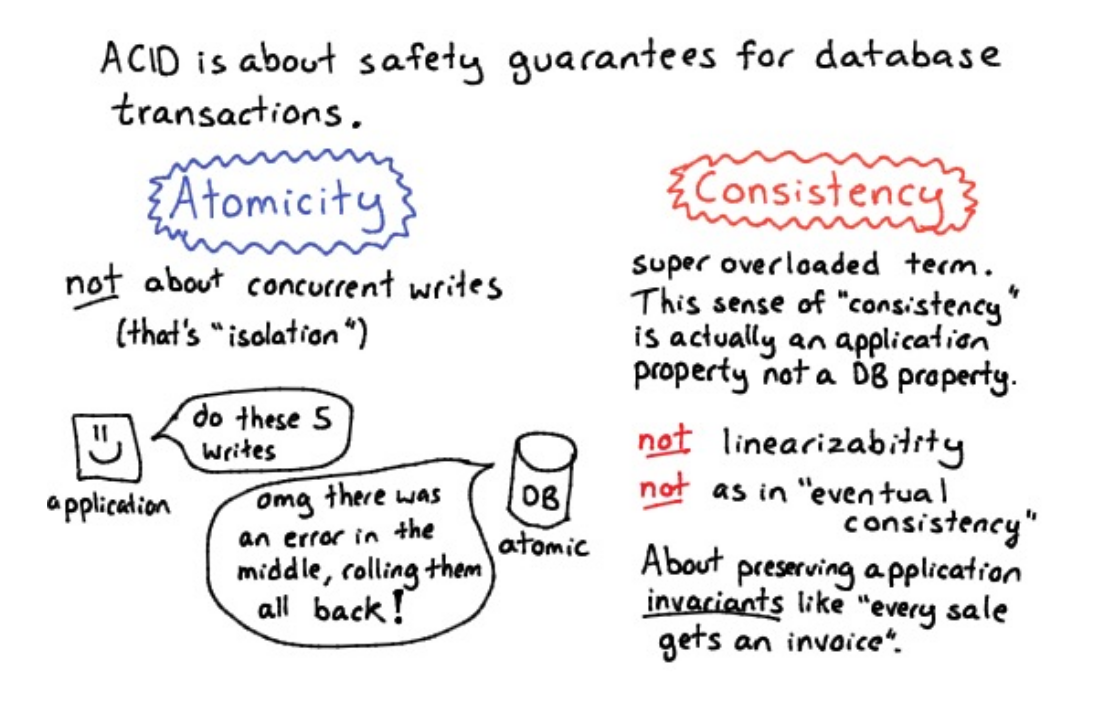
\includegraphics[scale=0.3]{2}
  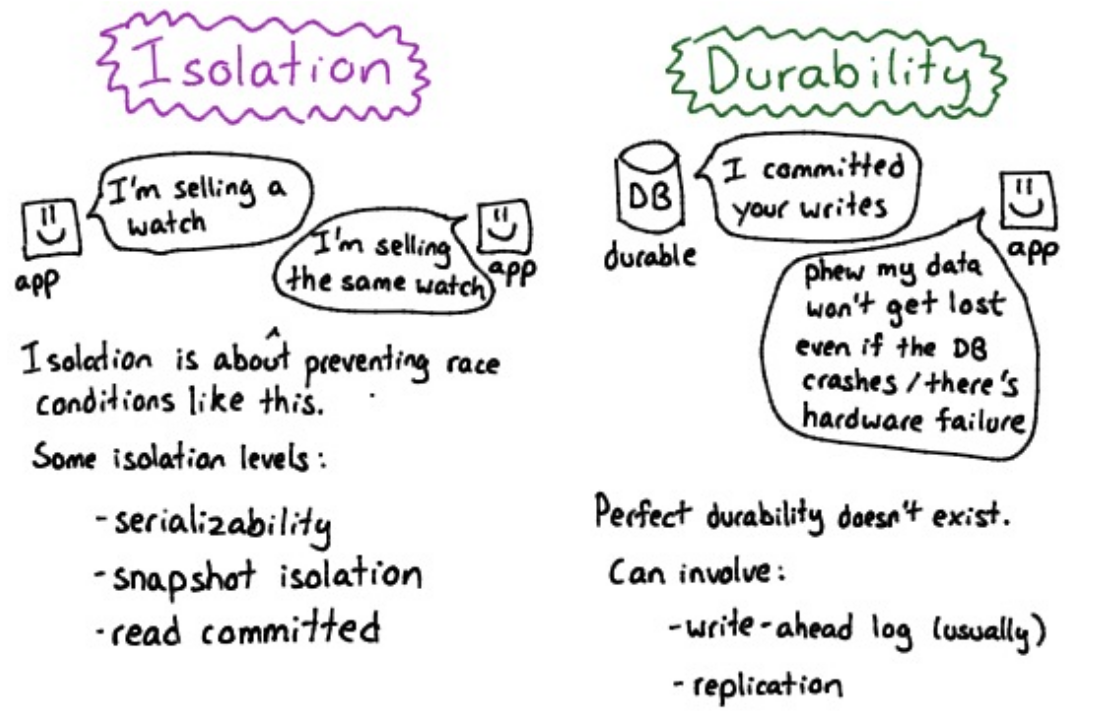
\includegraphics[scale=0.3]{3}
\end{center}

(Ver slides 7-8, história das bases de dados relacionais)

\pagebreak


\subsection{Current Trends and Issues}

\begin{flushleft}
  Algumas trends e issues motivaram à mudança nas tecnologias de armazenamento
de dados relacionais (em use cases e na tecnologia).

\textbf{Key Trends include:} Aumentar o volume de dados e tráfego. Ligação entre dados mais complexo.
\textbf{Key Issues include:} O problema $\rightarrow$ \textbf{impedance mismatch}.
\end{flushleft}

\subsection{Impedance Mismatch}

Nos últimos tempos, tem-se assistindo a um \textbf{aumento do volume de dados e tráfego}, a par da
redução do relacionamento entre eles, ou seja, \textbf{cada vez há mais dados não relacionados}.

Tem-se também verificado um conflito entre os \uline{princípios de engenharia de
software}, onde o
paradigma é \uline{orientado a objetos} e os princípios relacionais baseados em \uline{modelos
matemáticos}. Este problema é designado por \textbf{Impedance} (oposição que um circuito elétrico faz à passagem de corrente elétrica quando é submetido a tensão)
\textbf{Mismatch} (Disparidade, incompatibilidade).

Atualmente, este verifica-se nas estruturas isoladas, que violam os princípios da \textbf{normalização}.
Para armazenar informação persistentemente em programas modernos, uma única
estrutura lógica tem de ser separada (\textbf{normalização}).

\subsubsection{Exemplo}

Vários objetos que representem funcionários numa empresa. Cada funcionário terá o seu departamento,
mas vários funcionários podem trabalhar no mesmo departamento. Se a base de dados refletir o paradigma orientado a
objetos, iremos ter uma repetição dos departamentos nos vários funcionários e base de dados não estará normalizada!

No entanto, fazer múltiplos selects e joins para construir uma entidade às vezes não é a melhor opção.

\begin{center}
  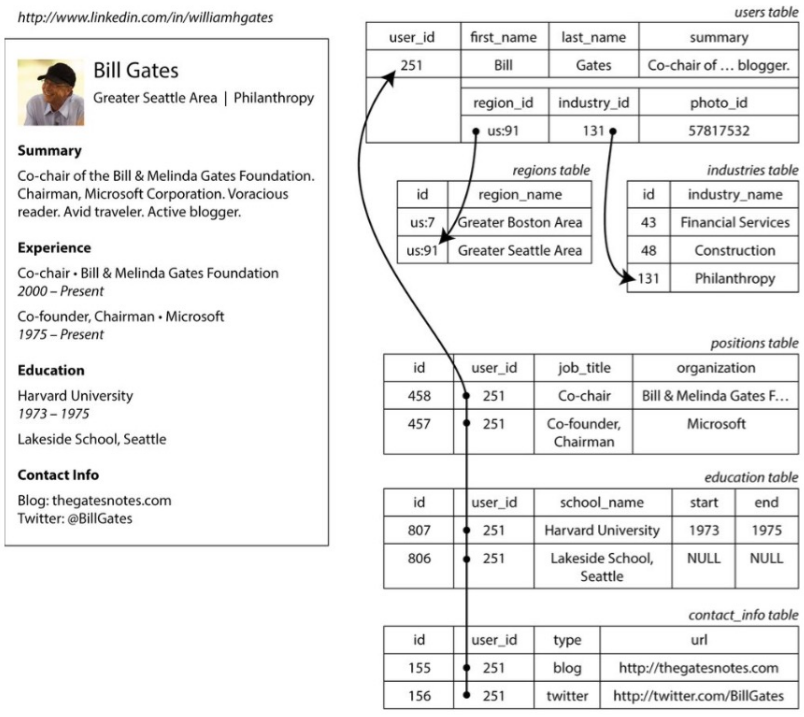
\includegraphics[scale=0.3]{4}
\end{center}

\pagebreak

\subsubsection{One-to-Many relations}

\begin{center}
  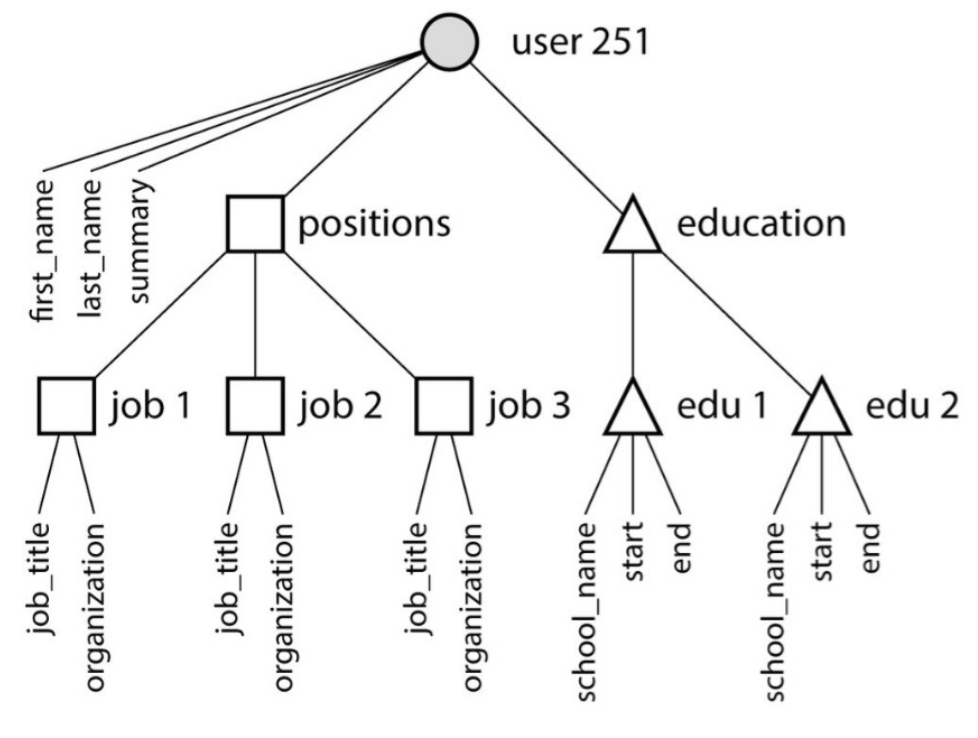
\includegraphics[scale=0.2]{5}
\end{center}

\subsection{Normalização}

Tem o objetivo de \textbf{reduzir a redundância dos dados}.
Em DB's este reflete-se na \uline{utilização de IDs} para identificar entidades,
oferecendo uma \textbf{consistência de utilização}, ao mesmo tempo que
\textbf{previne ambiguidades}, caso hajam entidades semelhantes (ex: com o mesmo nome),
\textbf{facilita alterações} das entidades, uma vez que a sua informação está armazenada
numa única tabela, motivo pelo qual também \textbf{facilita a tradução}.

\begin{flushleft}
  \textbf{Nota:} Uma base de dados que verifica estas características diz-se \textbf{normalizada}.
  Uma base de dados na qual as entidades como região e industria estão referidas
  por ID diz-se \textbf{normalizada}.

  No entanto, uma basde de dados que duplica nomes e propriedades de entidades
  em cada documento diz-se \textbf{desnormalizada}.
\end{flushleft}

\subsubsection{Many-to-Many relationships}

\begin{center}
  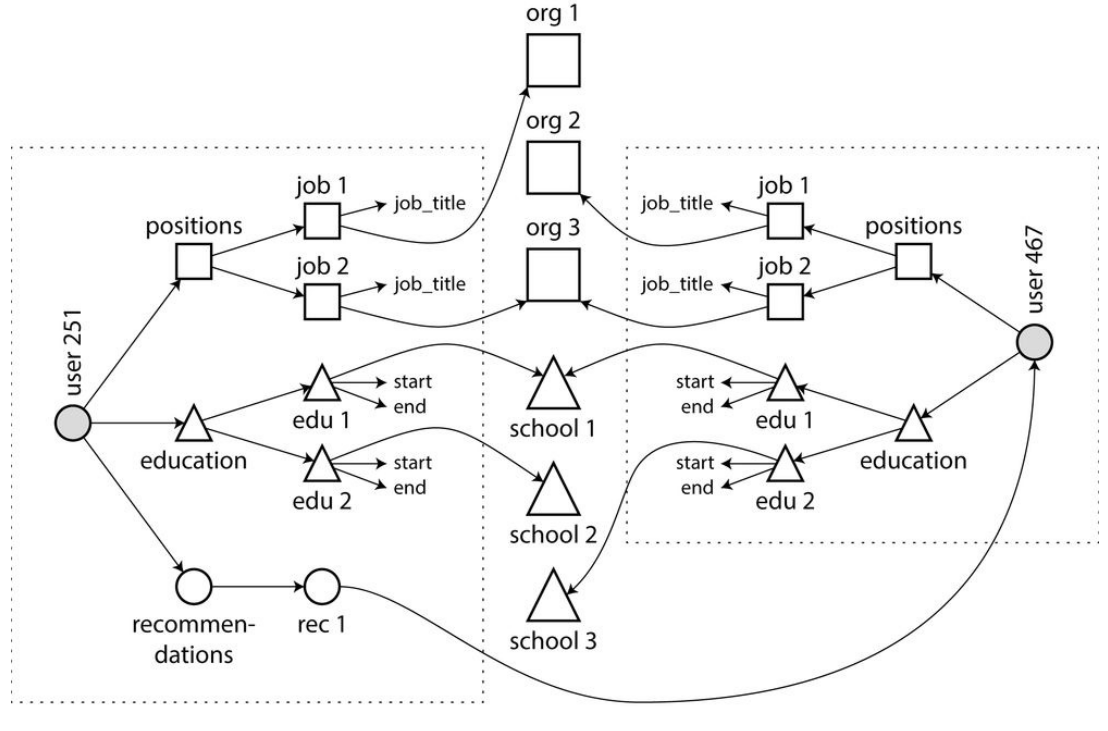
\includegraphics[scale=0.25]{6}
\end{center}

\pagebreak

\subsection{Responder ao aumento do volume de dados}

We are creating, storing, processing more data than ever before!

\vspace{3mm}
Existem duas abordagens possíveis:
\begin{itemize}
  \item Contruir bases de dados mauores;
  \item Criar um grupo de máquinas mais pequenas que se complementam;
\end{itemize}

\begin{enumerate}
  \item A primeira abordagem tem alguns problemas, uma vez que o \textbf{custo}
  de duplicar a capacidade de uma DB é geralmente mais do dobro do custo de uma
  DB "normal" e mesmo com recursos financeiros, há \textbf{limitações físicas} e de
  engenharia à sua capacidade;
  
  \item A segunda, apesar de mais exequível, tem também alguns defeitos, uma vez
  que por ser uma solução \textbf{barata}, pode refletir-se em \textbf{menos
  fiabilidade}. É ainda nexessário a integração com um DBMS compatível com
  a tipologia.
\end{enumerate}

Os Sistemas de Gestão de Bases de Dados (DBMS) têm alguma \textbf{dificuldade em gerir a escalabilidade
horizontal} (distribuição da BD).

\subsection{O movimento NoSQL}

Este movimento, cujo acrónimo significa
\textbf{Not only SQL}, pretende promover a utilização de bases
de dados não relacionais (SQL). Tem por base vários princípios.

\begin{enumerate}
  \item \textbf{Não é relacional} - Podem ser mas não são boas nisso;
  \item \textbf{API simples} - Sem necessidade de realizar \uline{join};
  \item \textbf{Teorema BASE \& CAP} - Viola os princípios ACID;
  \item \textbf{Schema-free} - Esquema implícito e gerido pela aplicação (sem verificações do lado da DB);
  \item \textbf{Distribuídas} - Algumas mais do que outras;
  \item \textbf{Open-source} - Mostly;
\end{enumerate}

\subsubsection{Transações BASE}

Este acrónimo nasceu em oposição aos princípios ACID, principalmente
em resposta às limitações de consistência que um cenário de um sistema
distribuído impõe.

\begin{itemize}
  \item \textbf{\uline{B}asic \uline{A}vailability} - A DB funciona a maior parte do tempo;
  \item \textbf{\uline{S}oft-state} - As manipulações dos dados não têm de ser write-consistent, nem
  diferentes réplicas têm de ser mutualmente consistentes o tempo todo.
  Escritas num nó da base de dados não têm de ser escritas garantidamente em simultâneo nos restantes nós;
  \item \textbf{\uline{E}ventual consistency} - O armazenamento de dados eventualmente torna-se consistente, em algum ponto
  (e.g. lazily at read time);
\end{itemize}

As bases de dados NoSQL caracterizam-se então por ser \textbf{otimistas} e \textbf{simples}, o que torna a
base de dados mais \textbf{rápida}, \textbf{disponibilidade em primeiro lugar}, \textbf{best effort} e \textbf{appoximate answers OK}.

\pagebreak

\subsubsection{Teorema CAP (Brewer's)}

Este teorema diz que um sistema distribuído só pode apresentar duas de três características:

\begin{itemize}
  \item \textbf{\uline{C}onsistent} - Escritas atómicas em toda a DB em simultâneo;
  \item \textbf{\uline{A}vailable} - A DB responde sempre a pedidos;
  \item \textbf{\uline{P}artition Tolerant} - O sistema consegue funcionar mesmo que um nó deixe de responder;
\end{itemize}

\begin{center}
  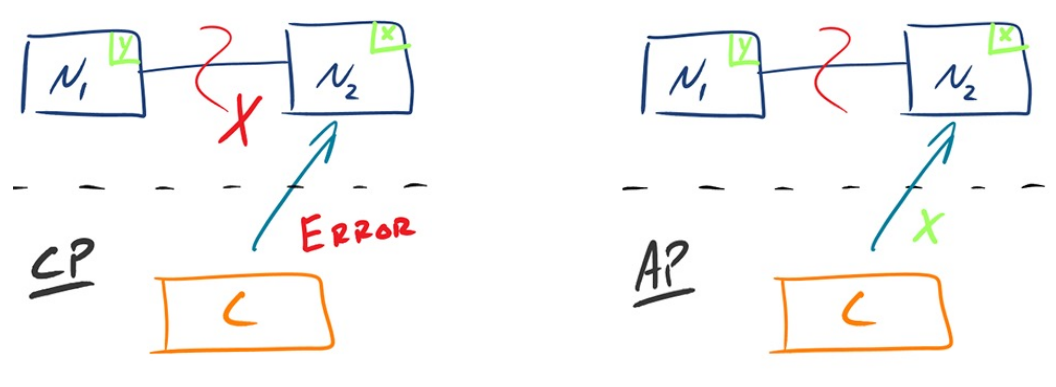
\includegraphics[scale=0.3]{7}
\end{center}

\begin{flushleft}
  \begin{enumerate}
    \item No primeiro temos uma base de dados que implementa a consistência e a tolerância a falhas.
    Quando um cliente faz um pedido de consulta de um valor, caso o nó não consiga contactar os restantes de forma a
    confirmar que todos têm o mesmo valor, retorna uma mensagem de erro.
    \item No segundo temos a disponibilidade e tolerância a falhas. Neste caso, mesmo com uma falha de comunicação entre
    os nós, o nó contactado pelo cliente vai responder com o valor pedido, mesmo que este não seja o mai atual.
  \end{enumerate}
\end{flushleft}

\begin{center}
  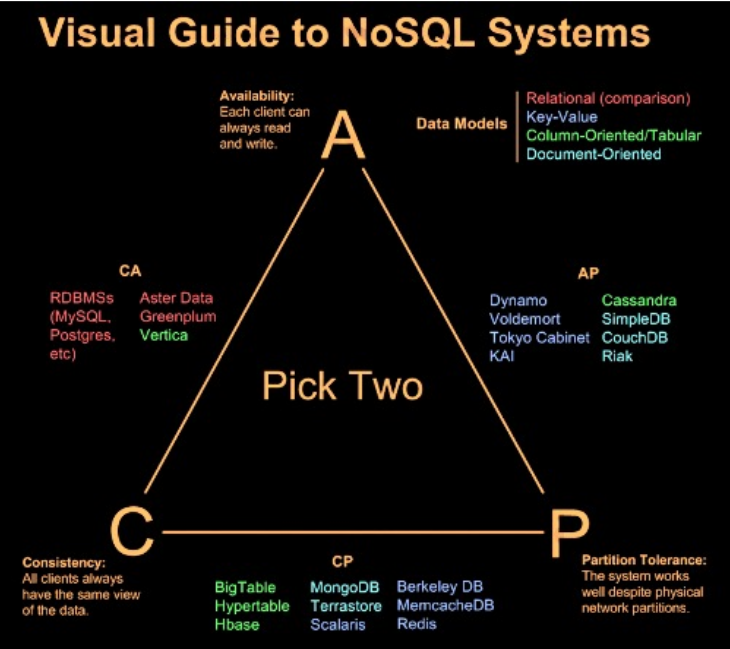
\includegraphics[scale=0.3]{8}
\end{center}

\pagebreak

\subsection{Tipos de Bases de Dados NoSQL}

\begin{flushleft}
  Existem vários tipos de bases de dados NoSQL. Core types:
  \begin{itemize}
    \item \textbf{Key-value stores}
    \item \textbf{Document stores}
    \item \textbf{Column stores}
    \item \textbf{Graph databases}
  \end{itemize}

  Non-core types:
  \begin{itemize}
    \item \textbf{Object databases}
    \item \textbf{Native XML databases}
    \item \textbf{RDF stores}
    \item \textbf{\dots}
  \end{itemize}
\end{flushleft}

\subsubsection{Key-value Databases}

Esta base de dados está focada em \textbf{armazanamento chave-valor}. É a mais simples
e funciona como uma simples hash table, tabela de dispersão (mapping).

\begin{flushleft}
  \textbf{Chave} - Identificador (chave primária) único, normalmente uma string;
  
  \textbf{Valor} - Pode assumir uma variedade de tipos, desde texto a estruturas de dados, \dots;
\end{flushleft}

As \uline{operações} são realizadas \uline{sobre um valor} de uma determinada chave.

A sua \textbf{simplicidade} permite uma boa \textbf{performance} e facilidade na \textbf{escalabilidade}. No entanto,
\uline{não permite} a realização de
queries complexos nem o armazenamento de dados complexos.
Usadas para perfis de utilizadores, informações de sessão, carrinhos de compras, preferências do utilizado, \dots

Tipicamente armazenam \uline{dados não persistentes}. \uline{Não permitem relações entre entidades}.
Não usar quando existem relações entre entidades, ou quando as queries pretendem
ter acesso aos valor.

\subsubsection{Document Databases}

O modelo de dados é uma estrutura complexa (tipicamente JSON ou XML), \textbf{self-describing},
uma vez que o nome dos atributos se descreve a si próprio, organizadas
numa \textbf{estrutura hierárquica} e onde cada documento tem um \textbf{identificador único}.

Pertmitem \uline{queries} sobre vários documentos, não só pela sua chave (id),
mas também pelo seu valor. É possível contruir índices, nos query patterns
podemos criar, atualizar e remover documentos, bem como é possível fazer
pesquisa usando queries complexas.

Quando comparadas com as bases de dados chave-valor, estas são uma evolução,
em que o valor é examinavél.

\begin{center}
  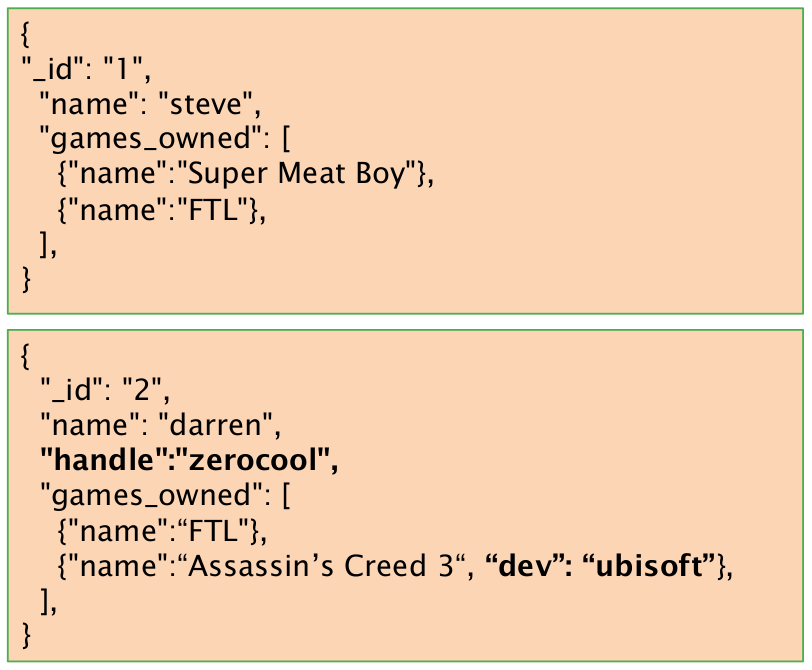
\includegraphics[scale=0.2]{9}
\end{center}

\begin{flushleft}
  \textbf{Usar:} Log de eventos, blogs, sistemas de gestão de conteúdos,
  web analytics, aplicações e-commerce, \dots
  \textbf{Documentos estruturados com um schema semelhante}.

  \textbf{Não usar:} Operações de \textbf{set} que envolva múltiplos documentos,
  onde o design da estrutura do documento esteja sempre a mudar e
  em relações \textbf{many-to-many}.
\end{flushleft}

\subsubsection{Column Databases}

\begin{flushleft}
  \textbf{Data Model:}
  \begin{itemize}
    \item \textbf{Familia de Colunas (Table)}
    \begin{itemize}
      \item Table é uma coleção de rows similares (mas não necessariamente identicas);
    \end{itemize}
    \item \textbf{Row}
    \begin{itemize}
      \item Coleção de colunas - deve compactar um grupo de dados a ser acedidos juntos;
      \item Associado a uma chave única de row (row key);
    \end{itemize}
    \item \textbf{Column}
    \begin{itemize}
      \item Consiste no nome da coluna, valor da coluna (possivelmente outros metadados)
      \item Valores escalares, sets flat, listas ou maps;
    \end{itemize}
  \end{itemize}

  \textbf{Query Patterns:}
  \begin{itemize}
    \item Criar, atualizar ou remover row de uma dada familia de colunas;
    \item Selecionar rows de acordo com a row key ou outras condições simples;
  \end{itemize}

  \textbf{Use Cases:}
  \begin{itemize}
    \item Event logging, content management systems, blogs, \dots
    \item Basicamente tudo o que for structured flat data com um schema parecido
    \item Batch processing via MapReduce;
  \end{itemize}

  \pagebreak

  \textbf{Quando NÃO usar:}
  \begin{itemize}
    \item Precisamos de ACID transactions;
    \item Queries complexas (aggregation, joins, \dots);
    \item Prototipos iniciais (quando o design da bd ainda está sujeita a mudanças)
  \end{itemize}
\end{flushleft}

\subsubsection{Graph Databases}

\begin{flushleft}
  \textbf{Data Model:}
  \begin{itemize}
    \item Foco na modelação da estrutura e propriedade dos grafos;
    \item Grafos podem ser ou não direcionados;
    \item Grafos são coleções de:
    \begin{itemize}
      \item Nós (vertices) para entidades do mundo real;
      \item Relações (edges) entre estes nós;
    \end{itemize}
    \item Ambos os nós e relações podem ter propriedades;
  \end{itemize}

  \textbf{Query Patterns:}
  \begin{itemize}
    \item Criar, atualizar ou remover nós/relações do grafo:
    \begin{itemize}
      \item Algoritmos de Grafos
      \item General Graph Traversal
      \item Sub-Graph ou Super-Graph Queries
      \item Similarity based Queries
    \end{itemize}
  \end{itemize}

  \textbf{Use Cases:}
  \begin{itemize}
    \item Social networks, routing, dispatch, location based services, \dots
  \end{itemize}

  \textbf{Quando NÃO usar:}
  \begin{itemize}
    \item Quando operações extensivas de batch são necessárias (múltiplos nós/relações
    são afetadas);
    \item Vamos dar store de grafos demasiado grandes (a distribuição de grafos ou até mesmo impossível);
  \end{itemize}
\end{flushleft}

\pagebreak

\subsubsection{Native XML Databases}

\begin{flushleft}
  \textbf{Data Model:}
  \begin{itemize}
    \item Documentos XML;
    \item Estrutura em árvore com nested elements, atributos e valores de texto;
    \item Documentos organizados em coleções;
  \end{itemize}

  \textbf{Query Languages:}
  \begin{itemize}
    \item Xpath (XML Path Language);
    \item XQuery (XML Query Language);
    \item XSLT (Extensible Stylesheet Language Transformations);
  \end{itemize}
\end{flushleft}

\subsubsection{RDF Databases}

\begin{flushleft}
  \begin{itemize}
    \item RDF Triples
    \begin{itemize}
      \item Subject, Predicate, Object;
      \item Cada Triple representa uma statement sobre uma entidade do mundo real;
    \end{itemize}
    \item Triples podem sser vistas em grafos
    \begin{itemize}
      \item Vertices representam os subjects e objects;
      \item Edges correspondem diretamente às statements individuais;
    \end{itemize}
  \end{itemize}

  \textbf{Query Languages:}
  \begin{itemize}
    \item SPARQL (SPARQL Protocol and RDF Query Language);
  \end{itemize}
\end{flushleft}

\subsubsection{Databases and data connectivity}

\begin{center}
  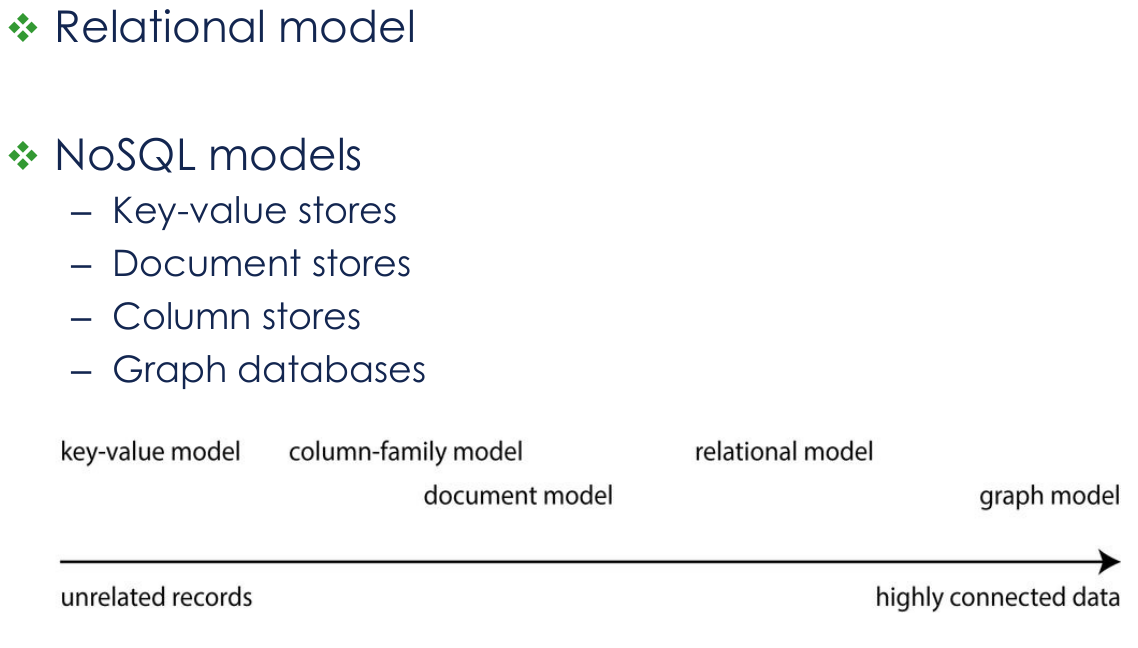
\includegraphics[scale=0.25]{41}
\end{center}

\pagebreak

\subsubsection{Considerações Finais}

As NoSQL DBs \textbf{NÃO} são o fim das bases de dados relacionais.
Estas continuam a ser preferiveis para 90\% dos projetos, para além do facto
das pessoas estarem mais familiarizadas, serem mais estáveis, terem mais
fearures e mais documentação e suporte disponível.

Mesmo assim devemos considerar diferentes modelos e sistemas de bases de dados.

\vspace{2mm}

\begin{flushleft}
  \textbf{Persistência Poliglota} - Uso de diferentes data stores em diferentes circunstâncias.
\end{flushleft}

\section{Armazenamento e recolha de dados}

Até aqui as bases de dados foram analisadas da perspetiva do utilizador, de quem armazena
dados e opera sobre eles. No entanto, a escolha de uma base de dados para um projeto
implica um conhecimento mais profundo sobre o seu modo de funcionamento interno.

Neste capítulo será explorada em detalhe a forma como as bases de dados armazenam e
obtêm os dados e distinguidas as bases de dados otimizadas para trabalhos transacionais das
otimizadas para analíticos.

\subsection{Append-only log: Um exmplo em bash}

O script abaixo define uma base de dados em bash.

\begin{lstlisting}
  #!/bin/bash

  cbd_set () { echo "$1,$2" >> database }

  cbd_get () { grep "^$1," database | sed -e "s/^$1,//" | tail -n 1 }

  # Usage: $ cbd_set <key> <value> $ cbd_get <key>
\end{lstlisting}

Este limita-se a adicionar a um ficheiro (append) um par chave/valor em cada
linha através da função cbd\_set e a filtrar o seu conteúdo para as linhas que
contenham a chave no cbd\_get, mostrando a última correspondência (chave mais
recente). É um ficheiro de texto simples, em que cada linha é um par chave/valor
separados por vírgula. Uma call ao cbd\_set acrescenta uma linha ao ficheiro,
sendo que versões anteriores não são overwriten.

\begin{lstlisting}
  $ cbd_set 42 '{"name":"San Francisco","attractions":["Exploratorium"]}'

  $ cbd_get 42
  {"name":"San Francisco","attractions":["Exploratorium"]}

  $ cat database
  123456,{"name":"London","attractions":["Big Ben","London Eye"]}
  42,{"name":"San Francisco","attractions":["Golden Gate Bridge"]}
  42,{"name":"San Francisco","attractions":["Exploratorium"]}
\end{lstlisting}

\pagebreak

Uma vez que não altera o conteúdo do ficheiro, limitando-se apenas a acrescentar-lhe linhas no
final, a função de inserção tem uma \textbf{excelente perfomance, O(1)}, que é independente do
tamanho da base de dados.

Por outro lado, as consultas são \textbf{pouco eficientes} uma vez que obrigam à consulta de todo o
ficheiro à procura da chave mais recente que corresponda. Apresenta por isso um
desempenho \textbf{O(n)}. Para um função extremamente simples tem uma boa performance.
Muitas bases de dados usam uma append-only data file ou logs. O problema é quando a DB cresce.

Para encontrar eficientemente o valor de uma chave, precisamos de uma
estrutura de dados diferente: um índice.
\begin{itemize}
  \item Um índice é uma estrutura de dados adicional que deriva dos dados primários;
  \item Um índice bem escolhido aumentam a velocidade das queries, mas cada índice
  torna as operações de write mais lentas;
\end{itemize}

\begin{flushleft}
  \textbf{Nota:} A não repetição de chaves iria aumentar a eficiência da consulta uma vez que assim que encontrasse uma
  correspondência não precisava de continuar à procura da chave mais recente. No entanto, neste cenário a inserção iria
  ser prejudicada, uma vez que a alteração de uma linha implica a leitura e reescrita da totalidade do ficheiro, uma
  operação que é bastante mais dispendiosa que o
  append que faz atualmente.
\end{flushleft}

\subsection{Índices Hash}

Uma solução para \uline{aumentar a eficiência das consultas} são os \textbf{índices}, estruturas adicionais às
tabelas das BD que mantêm um mapeamento entre as chaves e a sua posição na base de
dados.

Key-value stores são tipo um dicionário, normalmente implementados como um hash map.
Uma estratégia simples de indexação: manter um in-memory hash map onde todas as keys
estão mapeadas para um byte offset no ficheiro de dados.

Isto é o que algumas key-store databases fazem (e.g. Bitcask, Riak, \dots).
Oferecem boa performance se o hash map for mantido em memória.

\begin{center}
  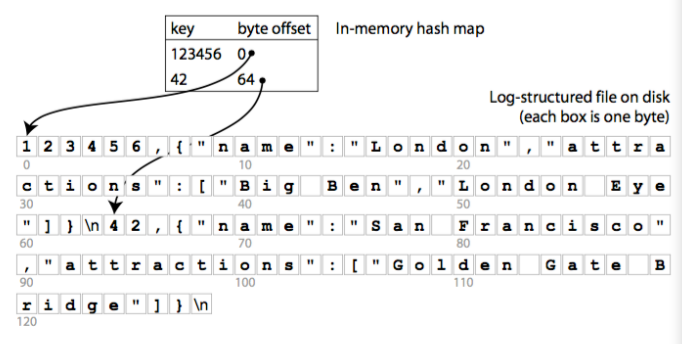
\includegraphics[scale=0.3]{42}
\end{center}

Apesar de agilizarem as consultas, \uline{prejudicam ligeiramente as inserções}, uma vez que para
além de registar os pares chave/valor é necessário atualizar também a sua localização nos
índices associados

\pagebreak

\subsection{Gestão do espaço em disco}

Uma base de dados como a analisada em que o conteúdo é sempre adicionado e nunca
reescrito vai ocupar cada vez mais espaço ao longo do tempo, aumentando também o tempo
das operações de consulta. A solução passa por \textbf{segmentar} e \textbf{compactar} e \textbf{combinar}.

\begin{flushleft}
  \textbf{Segmentar:} Em vez de utilizar um único ficheiro, utilizar vários (melhor performance).
  Cada segmento contém todos os valores escritos na DB num período de tempo.

  \vspace{2mm}

  \textbf{Nota: } Os ficheiros podem ter um tamanho máximo que quando é atingido faz com que os dados passem a ser armazenados
  num novo ficheiro. Com este modo de funcionamento pode inveter-se a pesquisa e começá-la pelos ficheiros mais
  recentes, evitando assim a análise de versões mais antigas da chave a ser procurada.
  O pior caso passa no entanto a ser menos eficiente, que é quando a chave tiver sido escrita apenas no primeiro ficheiro
  e nunca alterada, o que implica a análise de todos os ficheiros desde o mais recente ao mais antigo. Ao tempo da
  análise soma-se o tempo de abertura dos vários ficheiros

  \vspace{2mm}

  \textbf{Compactar:} Remove chaves duplicadas do log.

  \vspace{2mm}

  \textbf{Compactar e combinar:} Combinar os ficheiros antigos em versões mais compactas,
  mantendo apenas as versões mais recentes das chaves.

  \vspace{2mm}

  \textbf{Nota:} Esta operação pode ser realizada periodicamente por
  threads em background e não irá interferir com a
  disponibilidade da BD, uma vez que as operações são realizadas sobre os ficheiros mais recentes,
  que não estão a ser manipulados.

  \begin{center}
    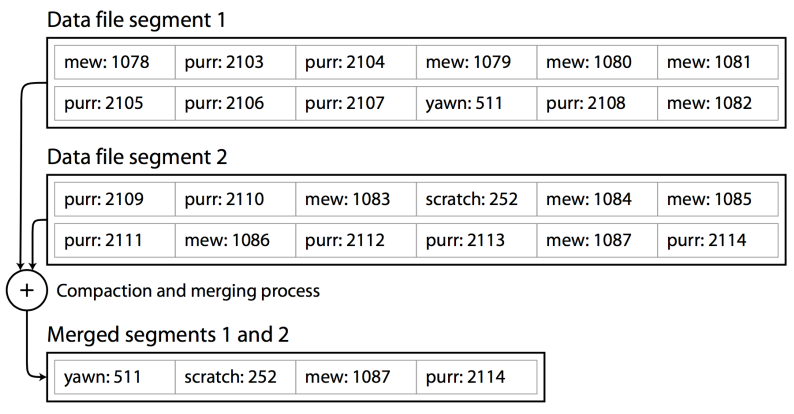
\includegraphics[scale=0.3]{43}
  \end{center}
\end{flushleft}

\subsection{Outros problemas}

Para além dos problemas analisados anteriormente há outros fatores que devem ser
considerados.

\vspace{2mm}

\begin{flushleft}
  O \textbf{formato de ficheiro} CSV não é o mais eficiente, sendo preferível a utilização de ficheiros
  binários.

  \vspace{2mm}

  Quanto à eliminação de registos, a remoção de todos os pares de uma chave em todos os
  ficheiros torna-se muito dispendiosa uma vez que como já foi mencionado implica a leitura e
  reescrita de todos os ficheiros alterados. A solução mais eficiente passa pela adição de um
  registo especial que indica a sua remoção (tombstone). Quando os segmentos do log são combinados,
  o processo discarta qualquer valor anterior para a chave eliminada.

  \pagebreak

  No que toca à \textbf{recuperação de falhas}, se o sistema utilizar estruturas de mapeamento (índices)
  em memória, o sistema irá demorar algum tempo a reconstrui-los em caso de falha do sistema
  uma vez que serão perdidos. A solução passa pela criação de
  snapshots em memória de cada hash map dos seguimentos (índice).

  \vspace{2mm}

  Há ainda a hipótese de \textbf{registos escritos parcialmente} caso o sistema falhe durante um
  processo de inserção. Uma solução possível é a implementação de checksums que permitem a partes
  corrompidas do log serem identificadas e ignoradas.

  \vspace{2mm}

  Por fim é ainda importante controlar o \textbf{acesso em concorrência} aos ficheiros. Sendo feita de
  forma sequencial, a \uline{escrita} deve ser feita apenas por uma
  thread única, enquanto que pelos
  dados serem imutáveis e
  append-only a \uline{leitura} pode ser feita em simultâneo por várias
  threads.
\end{flushleft}

\subsection{Append-only log}

O design append-only parece discartável À primeira vista, porque não dar update
aos dados do ficheiros dando overwrite aos valor antigo com o novo valor?

\vspace{2mm}

Acaba por ser bom por várias razões:
\begin{itemize}
  \item Dar append e combinar segmentos são operações de escrita sequanciais,
  que são muito mais rápidas que operações de escrita aleatórias;
  \item Concorrência e recuperação de falhas são muito mais simples se os ficheiros
  segmentados forem append-only ou imutáveis;
\end{itemize}

Mesmo havendo soluções para todos os problemas apresentados, há alguns que não têm
resolução, como a necessidade da
\textbf{hash-table caber em memória} (é dificil fazer um hash map on-disk que tenha
boa performance) e a dificuldade em fazer
\textbf{queries para intervalos de valores}.

\subsection{Sorted String Table (SSTable)}

Neste tipo de base de dados os pares chave/valor são ordenados pela chave, que é única (não
pode aparecer mais do que uma vez em cada ficheiro segmentado combinado, o processo
de combinar já faz isso).

\pagebreak

\subsubsection{Vantagens}

Aqui a \textbf{combinação} dos segmentos torna-se ainda mais \textbf{simples} e \textbf{eficiente}, uma vez que em cada segmento estarão os
pares cujas chaves estão próximas em termos de ordenação. Mesmo se os ficheiros
são maiores do que (tipo algoritmo mergesort).

Como consequência os \textbf{índices} tornam-se menos densos porque deixam de ter a necessidade
de indexar todas as chaves e passam a integrar apenas os padrões que identificam o início de
cada segmento (por exemplo “aa”, “br”, “h”).

A segmentação deve ser um compromisso entre ter o menor número de blocos possível e ter blocos o
mais pequenos possível

\begin{center}
  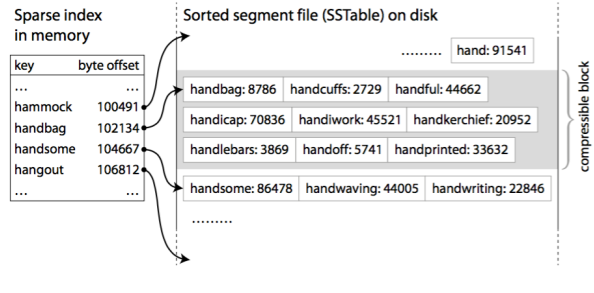
\includegraphics[scale=0.3]{44}
\end{center}

\subsubsection{Combinação de segmentos da SSTable}

\begin{center}
  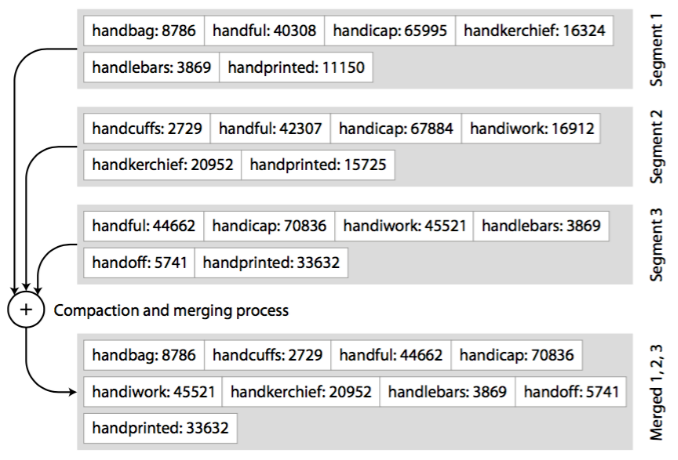
\includegraphics[scale=0.3]{45}
\end{center}

\subsubsection{Ordenação}

Quando a estrutura em árvore em memória (memtable) atinge um determinado limite, esta pode ser
armazenada em disco gerando um novo segmento.
\begin{itemize}
  \item Pode ser feito eficientemente porque os dados já estão ordenados nos pares key-value;
  \item A novo file SSTAble torna-se o segmento mais recente da DB;
  \item Quando a noca SSTable está pronta, a memtable pode ser esvasiada; 
\end{itemize}

\vspace{2mm}

As \uline{consultas analisam primeiro a árvore binária e se não encontrarem vão procurar no
segmento mais recente}, regredimento depois no tempo até encontrar uma correspondência.

\vspace{2mm}

Esta abordagem, apesar de agilizar os processos de escrita prejudica os de leitura. Deve para
evitar isto ser aplicada periodicamente a \textbf{combinação} e \textbf{compactação}.

\pagebreak

\subsubsection{Recuperação a falhas}

Uma vez que os dados mais recentes são armazenados em memória, em caso de falha do
sistema serão perdidos. Para evitar este problema, muitas SST mantém um \textbf{append-only log} em
memória, que atualizam em cada escrita, de forma a permitir esta recuperação.

\subsection{B-trees}

Este é o mecanismo de indexação mais comum em sistemas de bases de dados. Tal como as
SST estudadas anteriormente, as B-trees mantêm os pares chave/valor ordenados pela chave,
o que torna as \textbf{leituras bastante eficientes}, mesmo com
\uline{queries com intervalos}.

As B-trees partem a Db em blocos/páginas de tamanho fixo,
tradicionalmente 4KB, e a leitura e escrita numa página de cada vez.
Facilita o seu armazenamento uma vez que estão em sintonia com o
hardware.

\begin{center}
  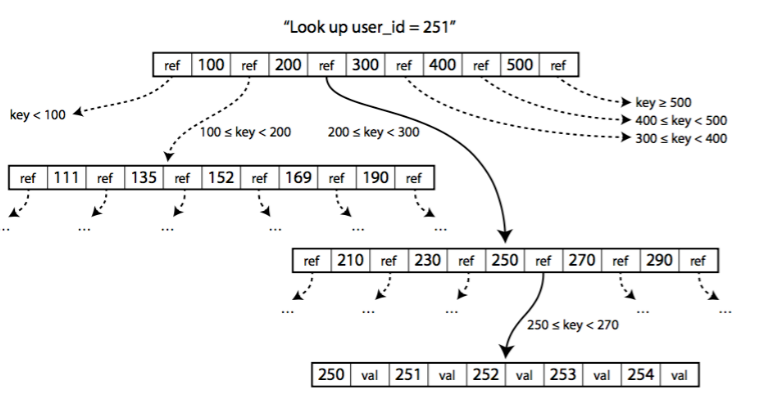
\includegraphics[scale=0.3]{46}
\end{center}

\begin{flushleft}
  \textbf{Nota:} Na camada do
  hardware os discos também são compostos por blocos de
  tamanho fixo.
\end{flushleft}

A estrutura começa pela página raiz.

Em cada página há k valores e k+1 referências a outras
páginas, sendo k geralmente um valor na ordem das
centenas.

Cada filho é responsavél por um intervalo continuo de chaves, e as chaves
da página root indicam os intervalos de chaves dos filhos.

\subsubsection{Operações}

As operações de \textbf{pesquisa}, \textbf{inserção} e \textbf{remoção} são de complexidade $O(log_k n)$.

A \textbf{inserção} é a operação com maior custo, uma vez que no caso de ser feita numa página que
já tenha atingido o tamanho k, obriga à sua divisão em duas páginas e à reoganização dessa
área da árvore, que pode impactar várias páginas.

\textbf{Atualizar} um valor de uma key já existente:
Pesquisar pela leaf page que contém a key e atualizar o valor. Escrever
a página de volta para o disco (qualquer referência a esta página permanece válida).

A árvore permanece balanceada.

\pagebreak

\subsubsection{Split numa página}

\begin{center}
  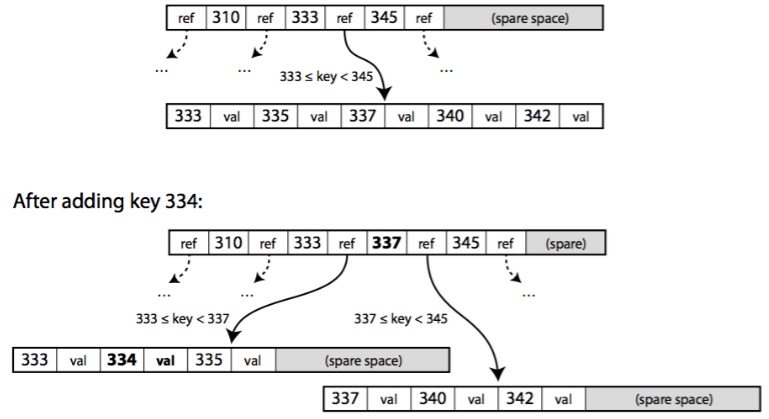
\includegraphics[scale=0.3]{47}
\end{center}

\subsubsection{Aspetos a considerar}

A \textbf{gestão de falhas} pode ser feita tal como nas SST com append-only logs.

A \textbf{gestão de concorrência} torna-se também fundamental, uma vez que não são desejáveis
escritas em simultâneo. Utilizam-se semáfros.

\subsubsection{Otimização}

De forma a responder aos problemas endereçados no último tópico pode ainda ser aplicada a
técnica \textbf{copy-on-write scheme}, que consiste na criação de páginas novas cada vez que alguma vai ser reescrita,
mudando a referência da antiga para a nova apenas quando a última estiver concluída.

\begin{flushleft}
  \textbf{Nota:} Garanta-se assim que caso haja alguma falha no processo de escrita a integridade da base de dados não é
  comprometida (embora as atualizações que estavam a ser feitas possam ser perdidas) e ainda que podem continuar a
  haver leituras sobre os dados antigos com garantia de que a base de dados está integra durante o processo de cópia.
\end{flushleft}

Podem ainda ser aplicadas técnicas de \uline{abreviação das chaves}.

\subsubsection{B-tree versus LSM-trees}

LSM-trees são tipicamente mais rápidas para escritas,
enquanto que as B-trees são mais rápidas para leituras.

\vspace{2mm}

Um downside de um log-structured storage é que o processo compactação
pode interferir com a performance de ongoing leitura e escritas.

\vspace{2mm}

Nas B-trees cada key existe apenas uma vez no índice, enquanto que
num log-structured storage pode ter várias cópias de diferentes segmentos.
\begin{itemize}
  \item Isto faz com que as B-trees sejam melhores para DB's que
  querem oferecer semânticas de transações fortes;
  \item Em muitas DB's relacionais, é implementado usando locks no range das keys,
  num índice B-tree, estes locks podem ser diretamente aplicados na árvore;
\end{itemize}

\pagebreak

\subsection{Outras estruturas de indexação}

Por vezes é útil a criação de \textbf{índices secundários} cujas \uline{chaves são atributos não únicos}. Podem
fazer corresponder a uma chave as suas várias referências (there
might be many rows (documents, vertices) with the same
key).

Pode ser feito de duas maneiras:
\begin{itemize}
  \item Fazer aos valores do índice um matching row identifiers (como um posting list in a full-text index);
  \item Tornar cada key única adicionando um identificador de row;
\end{itemize}

Os índices B-trees e log-structured podem ser usados como índices secundários. 

\vspace{2mm}

Há ainda cenários em que se justifica o \textbf{armazenamento dos valores no índice}, total ou
parcialmente. Tem limitações dependendo do espaço da memória. Facilitam a leitura, mas
prejudicam escritas.

\vspace{2mm}

Para situações em que seja necessário fazer
queries sobre várias colunas podem ser definidos
\textbf{índices multi-column}.

\vspace{2mm}

Todos os anteriores pressupõe a pesquisa por termos exatos. Os \textbf{índices fuzzy} fornecem uma
solução para \uline{pesquisas por similaridade}. Muito usado em pesquisas textuais (like).

\subsection{Manter tudo na memória}

Hoje em dia já existem bastantes bases de dados que funcionam baseadas em memória,
oferecendo redundância e persistência, ou seja, tolerantes a falhas

\vspace{2mm}

São geralmente mais rápidas que as suas homólogas (lados opostos), uma vez que não têm de codificar os
dados de forma a poderem ser armazenados em disco. Permitem por isso trabalhar com
estruturas que são difíceis de guardar em disco como
priority queues e sets.

\begin{flushleft}
  \textbf{Nota:} A rapidez não se deve por isso diretamente ao facto de não terem de escrever em disco, uma vez que as bases de
  dados em disco são geralmente carregadas em memória e acedidas a maior parte das vezes a partir da memória.
\end{flushleft}

\subsection{Processamento e análise transacional}

\subsubsection{Online Transaction Processing (OLTP)}

O \textbf{processamento transacional} define-se por permitir aos clientes fazer leituras e escritas com
baixa latência. As \uline{bases de dados que seguem este padrão de acesso} dizem-se \textbf{OLTP} (padrão de acesso).

Contrasta com o \textbf{batch processing}, uma tarefa de processamento realizada periodicamente
(p.e. uma vez por dia) para algum fim.

\pagebreak

\subsubsection{Online Analytic Processing (OLAP)}

Com a evolução das bases de dados, estas começaram a ser também utilizadas para \textbf{análise
de dados analíticos}, que geralmente consiste em ler e processar uma grande quantidade de
dados.

\begin{flushleft}
  \textbf{Nota:} Do ponto de vista técnico a construção do
  query não é complexa, mas a tarefa em si pode tornar-se dependendo do
  volume de dados em análise, que pode levar algum tempo a ser processado. Pode ainda haver o cenário em que um
  query para dados do ano anterior ser feito várias vezes, desnecessariamente uma vez que os dados não vão mudar.
\end{flushleft}

\subsubsection{OLTP vs OLAP}

O \textbf{OLTP} faz leituras de poucos registos de cada vez e de acesso aleatório, tal como a escrita,
que deve ter uma baixa latência. Os dados, utilizados maioritariamente pelo segmento
operacional das empresas, devem estar sempre atualizados e ocupam gigas.

\vspace{2mm}

Já no \textbf{OLAP} a leitura é feita em massa e a escrita em
bulk import, sobre dados históricos, que
ocupam teras. É utilizado pro gestores como suporte às suas tarefas de controlo e
planeamento.

\begin{center}
  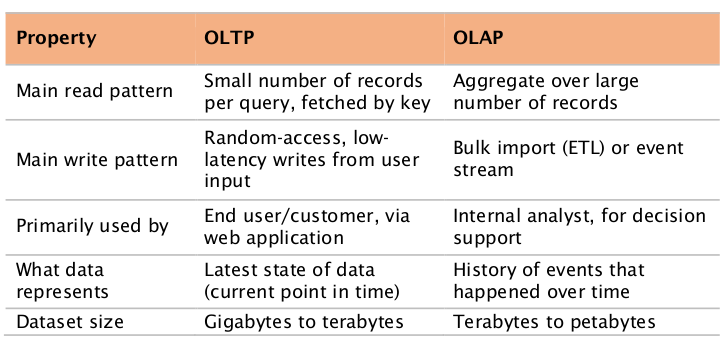
\includegraphics[scale=0.3]{48}
\end{center}

RDBMS e SQL trabalham bem com OLTP-type queries e com OLAP-type queries.

Os sistemas OLAP geralmente ocupam mais espaço que os OLTP porque não apresentam
normalização dos dados, ou seja, não tiram partido das características relacionais.

Dadas as suas características distintas, estes padrões são geralmente \uline{implememtados por
bases de dados distintas}.

As focadas em OLTP dizem-se \textbf{relacionais}, enquanto que as OLAP se dizem \textbf{data warehouses}.

\pagebreak

\subsection{Data Warehouse}

Estas bases de dados focadas na análise de dados \uline{geralmente estão associadas às
transacionais}, das quais \textbf{extraem} os dados, que são \textbf{transformados} e \textbf{limpos} antes de
\textbf{carregados}.

\begin{center}
  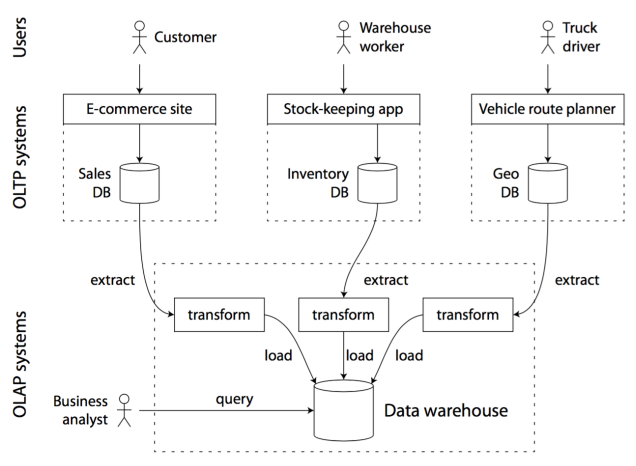
\includegraphics[scale=0.3]{49}
\end{center}

Este processamento é conhecido por \textbf{ETL} (
Extract, Transform, Load).

\vspace{2mm}

Os dados podem ser provenientes de várias bases de dados e ser \textbf{transformados} de forma a ser integrados de forma
unificada. Pode ainda ser feita uma \textbf{limpeza} eliminando registos nulos ou não consistentes.

\subsubsection{Porquê separa Data Warehouse}

\begin{flushleft}
  Porquê combinar OLTP e OLAP?
  \begin{itemize}
    \item Data warehouse são normalmente relacionais, porque SQL é bom para analytic queries.
    \item Muitas ferramentas OLTP (querying, visualization, \dots)
  \end{itemize}

  Porquê separar?
  \begin{itemize}
    \item Diferentes duncções e diferentes dados;
  \end{itemize}

  Muitos vendedores suportam ou transaction
  processing or analytics workloads.
\end{flushleft}

\pagebreak

\subsection{Esquema da base de dados}

O esquema destas bases de dados é conhecido por esquema em estrela (\textbf{star schema}) e consiste numa
tabela (entidade) principal, designada por \textbf{fact table}, onde cada linha corresponde a um evento num determinado tempo e cada
atributo um valor ou referência a outra tabela.

Existe ainda um modelo alternativo chamado \textbf{snowflake}, em que divide as duas dimensões do
anterior em várias. É por isso mais normalizada, mas como consequência mais complexa de
utilizar. 

\begin{center}
  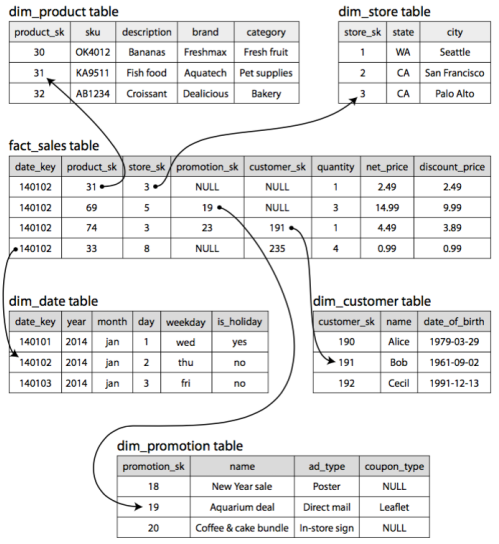
\includegraphics[scale=0.3]{50}
\end{center}

\subsection{Queries}

O facto de armazenar os dados históricos não normalizados leva a que as tabelas destas bases
de dados tenham um volume gigante de registos com um número muito elevado de colunas (fact tables
podem ter trilhões de rows e pentabytes de dados, normalmente têm mais de 100 colunas).
Isto não é um problema nas consultas às linhas, porque geralmente são apenas lidas poucas
de cada vez

\vspace{2mm}

No entanto, para obter todos os valores de uma coluna é necessário ler a totalidade da tabela,
desperdiçando imensos recursos, OLTP databases são row-oriented: todos os valores de uma row
estão próximos. Neste caso, a solução passa pelo \textbf{armazenamento orientado
às colunas}.

\pagebreak

\subsubsection{Armazenamento orientado a colunas}

Este tipo de armazenamento consiste em separar cada linha
pelas suas colunas e guardar cada coluna num ficheiro/bloco
separado. Tem por base o princípio que cada ficheiro tem as
\textbf{colunas de cada linha pela mesma ordem}
Se cada coluna estiver num ficheiro separado,
a query apenas precisa de ler e processar estas colunas.

Este tipo de armazenamento não é eficiente para leituras por linha!

\begin{center}
  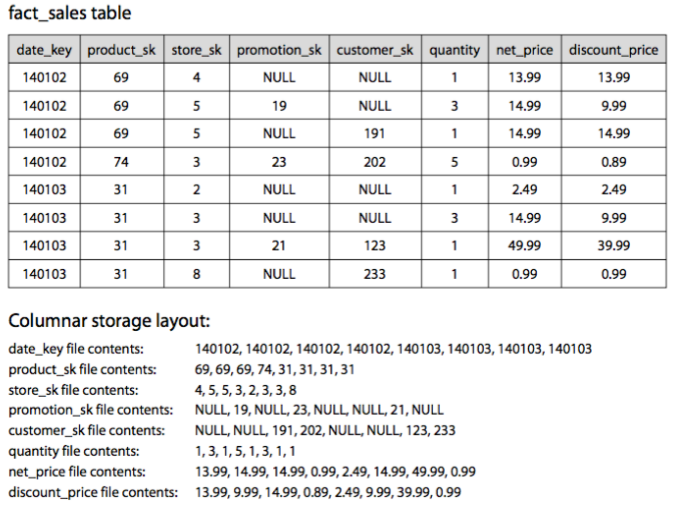
\includegraphics[scale=0.3]{51}
\end{center}

Devido à \textbf{homogeneidade entre os dados} da mesma coluna é facilitada a compressão.

Uma técnica que é particularmente efetiva em data warehouses é bitmap encoding.

\vspace{2mm}

A \textbf{ordenação} pode ser realizada por uma determinada coluna dependendo dos dados e do fim
a que se destinam, mas não esquecer que a mesma posição em todos os ficheiros tem de
corresponder à mesma linha, pelo que todos os ficheiros têm de ser reordenados.

\subsubsection{Escrita}

O armazenamento de column-oriented, a compressão e a ordenação ajudam
a fazer as queries OLAP mais rápidas.

Se os dados forem ordenados, a escrita de novos valores na BD torna-se um processo algo
complexo, de forma a garantir a consistência.

\vspace{2mm}

Em \uline{estruturas operacionais} que implementam este tipo de armazenamento geralmente opta-se
por \textbf{B-trees com append-log}. Uma boa solução é uma \textbf{LSM-tree}, que na prática é uma \textbf{SSTable}.

\begin{center}
  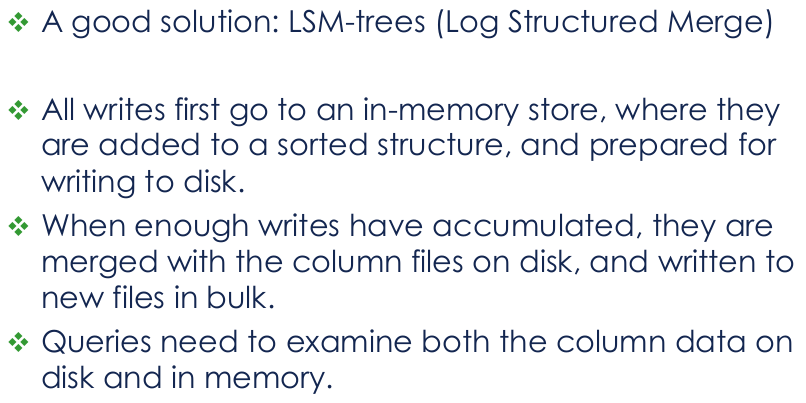
\includegraphics[scale=0.3]{52}
\end{center}

\pagebreak

\subsection{Materialized views}

Data warehouse queries often involve an
aggregate function (COUNT, SUM, AVG, MIN, ...).

\textbf{Materialized views} são um conjunto de agregações agrupadas em várias dimensões.

Dada a complexidade dos
queries de consulta às bases de dados OLAP, geralmente estas têm
a si associadas \textbf{data cubes ou OLAP cube}, um tipo de \textbf{materialized view}, que consistem numa tabela da base
de dados em
cache que armazena dados agregados para efeitos de eficiência.

\begin{center}
  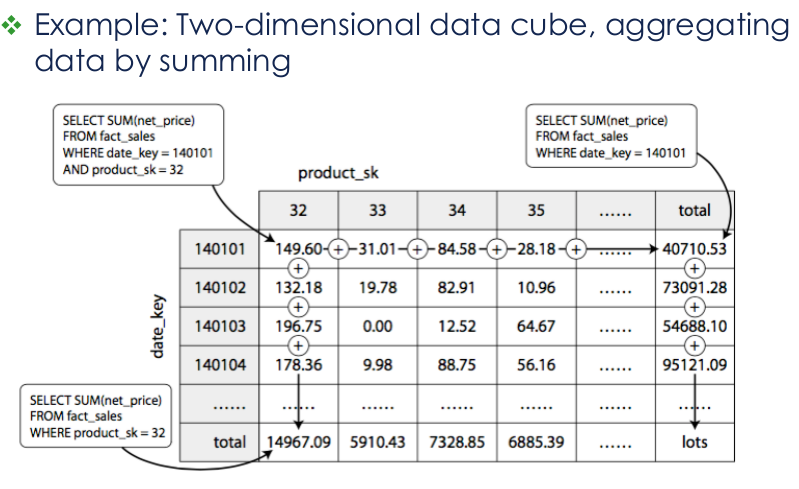
\includegraphics[scale=0.3]{53}
\end{center}

\section{Formatos de dados}

Aplicações inevitavelmente \textbf{mudam} ao longo do tempo, e em muitos casos
isto precisa de uma mudança nos dados.
Versões antigas e novas do código, e versões antigas e novas dos dados,
podem, potencialmente, coexistir no sistema ao mesmo tempo.

Para o sistema continuar a correr sem problemas, é necessário
manter compatibilidade em ambas as direções:

\begin{flushleft}
  \textbf{Backward compatibility -} Novo código pode ler dados que foram escritos
  pelo código antigo (novas versões podem ler dados antigos).

  \textbf{Forward compatibility -} Código antigo pode ler dados que foram escritos
  pelo novo código (versões antigas podem ler dados novos). Requere que o código antigo
  ignore adições feitas pela nova versão do código.
\end{flushleft}

Programas geralmente trabalham com dados\dots
\begin{itemize}
  \item In memory, os dados são mantidos em objetos, structs, arrays, hash tables, trees \dots
  \item Out of memory, para escrever dados para um ficheiro, ou mandá-lo pela rede
  (i.e diferentes sequancias de bytes).
\end{itemize}

A translação da representação in-memory para uma sequência de bytes é chamada de
\textbf{encoding}, \textbf{serialization} ou \textbf{marshalling}.

O inverso é chamado de \textbf{decoding}, \textbf{deserialization} ou \textbf{unmarshalling}.

\pagebreak

\subsection{Formatos específicos de linguagens}

Muitas linguagens de programação oferecem bibliotecas que permitem a realização deste
processo. No entanto, os mecanismos que oferecem estão muitas vezes acoplados a essa
linguagem (não permitem a leitura por outras) e dependentes da sua versão, pelo que devem
ser apenas aplicados em \textbf{soluções temporárias}.

\begin{flushleft}
  \textbf{Nota:} Java mapeia
  Serializable, Ruby
  Marshal e Python
  Pickle
\end{flushleft}

\subsection{Formatos textuais}

A alternativa a este modelo são os formatos textuais, que a \textbf{maior vantagem} é serem legíveis pelo ser
humano. No entanto têm alguns problemas uma vez que implementam menos restrições, que
geram alguma \textbf{ambiguidade} entre tipos de dados, nomeadamente
strings e números (JSON lida com isto, mas não integers).
CSV não tem um schema, a aplicação deve definir o significado de cada row e colun.

Apesar de tudo, JSON, XML e CSV são bastante utilizados e úteis em muitos cenários.

\subsection{Codificação binária}

A terceira alternativa consiste no armazenamento em formato binário, que apesar de não ser
legível pelo ser humano, é \textbf{mais compacto e lidos mais rapidamente}, uma vez que o esquema
nos indica os tipos de dados a ler, pelo que são lidos diretamente no seu formato.

Para um dataset pequeno, os ganhos não são significativos, mas com terabytes,
a escolha do formato pode fazer uma grande diferença.

Num formato textual este é lido por completo como uma
string e dependendo do seu tipo é depois convertido.

Os formatos mais utilizados são binários de JSON (BSON, BJSON, UBJSON, …).

\subsection{Formatos textuais}

\subsubsection{CSV (comma-separated values)}

Este formato é \textbf{pouco estandardizado}, uma vez que aceita \uline{dois tipos de separadores} (vírgula e
ponto e vírgula), \uline{não tem um formato
escape definido}, nem informação quanto à sua
codificação.

\subsubsection*{Exemplo}

\begin{center}
  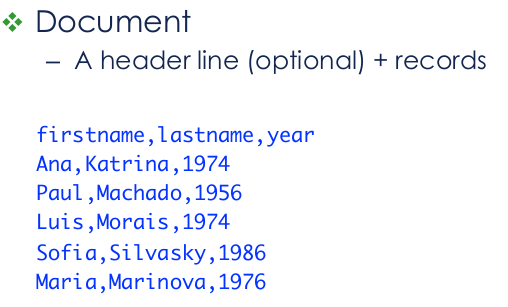
\includegraphics[scale=0.3]{54}
\end{center}

\pagebreak

\subsubsection{XML (Extensible Markup Language)}

Este formato é \textbf{semi-estruturado}, estando definidas normas quanto à forma como os dados são
organizados. Tem o objetivo de ser simples, generativo e usável na internet.

A sua estrutura é composta por \textbf{constructs}, que são delimitados pelos marcadores de abertura
e fecho, que podem ser do tipo vazio, textual, elemento (se tiverem
nested elements) ou uma
mistura dos anteriores.
Cada elemento pode estar associado com um conjunto de atributos.

Os atributos são feitos numa noção de \textbf{chave}(marcador)/valor.

Sequências de escape (entidades predefinidas), são usados dentro de valores de atributos
ou conteúdo textual de elementos. Ex: \&lt; é $<$, \&gt é $>$, \&quot é $"$, \dots

\subsubsection*{Exemplo}

\begin{center}
  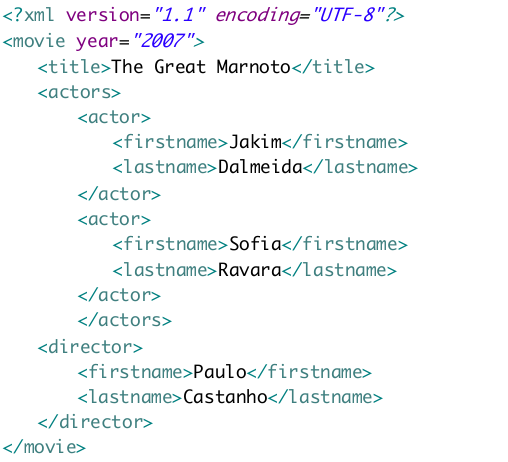
\includegraphics[scale=0.3]{55}
\end{center}

\subsubsection{JSON (JavaScript Object Notation)}

Este é um XML simplificado baseado na notação JavaScript (mas independente da linguagem), como sugerido pelo nome.

Objetivos:
\begin{itemize}
  \item Simplicidade: text-based, fácil de ler e escrever;
  \item Universal: estruturas de dados comuns (object e array);
\end{itemize}

JSON é construído em duas estruturas:

\begin{flushleft}
  \textbf{Coleção de pares chave/valor} - Em muitas linguagens, isto é caracterizado como um object, record, struct, dictionary,
  hash table, keyed list ou associative array.

  \textbf{Lista ordenada de valores} - Na maioria das linguagens, isto é caracterizado como um array, vector, list ou sequence.
\end{flushleft}

\pagebreak

\subsubsection*{Exemplo}

\begin{center}
  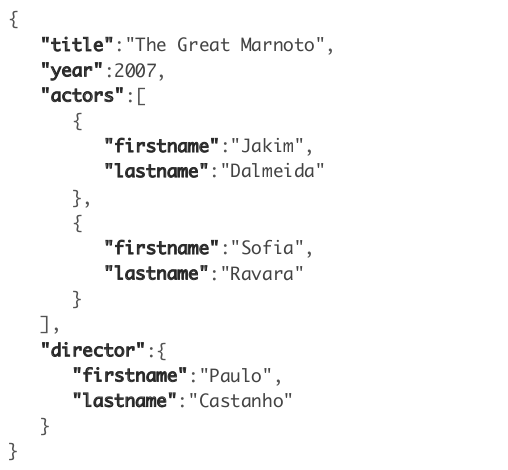
\includegraphics[scale=0.3]{56}
\end{center}

\subsubsection*{Estrutura de dados - Object}

Coleção não ordenada de pares chave/valor (propriedades). Corresponde a estruturas
como object, record, struct, dictionary, hash table, keyed list, associative array\dots

\begin{lstlisting}
  { "name": "John", "age": 22, "city": "London" }
  { }
\end{lstlisting}

\subsubsection*{Estrutura de dados - Array}

Coleção ordenada de valores. Corresponde a estruturas como array, vector, list, sequence\dots

Os valores podem ser de diferentes tipos, valores duplicados não são permitidos.

\begin{lstlisting}
  [ 2, 7, 7, 5 ]
  [ "John", 22, "London" ]
  [ ]
\end{lstlisting}

\pagebreak

\subsubsection*{Estrutura de dados - Value}

\begin{itemize}
  \item String unicode:
  \begin{itemize}
    \item Delimitada por aspas duplas;
    \item Sequências de escape: \textbackslash "a \textbackslash n b \textbackslash " c \textbackslash \textbackslash d;
  \end{itemize}

  \item Número:
  \begin{itemize}
    \item Inteiros decimais ou floats;
    \item Example: 42, -1.234, 6.02e23;
  \end{itemize}

  \item Nested object;
  \item Nested array;
  \item Boolean value: true or false;
  \item Missing information: null;
\end{itemize}

\subsubsection{BSON (Binary JSON)}

Binary-encoded serialization de JSON documents
\begin{itemize}
  \item Caracteristicas: Lightweight, \textbf{traversable}, efficient;
  \item \textbf{Armazenamento conveniente de informação binária} (bom para imagens e attachements);
  \item desenhado para fast in-memory manipulation;
  \item tipos de dados extra (para além de JSON): double, date, byte array, JS code,\dots
\end{itemize}

Usado pelo MongoDB:
\begin{itemize}
  \item NoSQL document database para documentos JSON;
\end{itemize}

\subsubsection*{Exemplo}

\begin{center}
  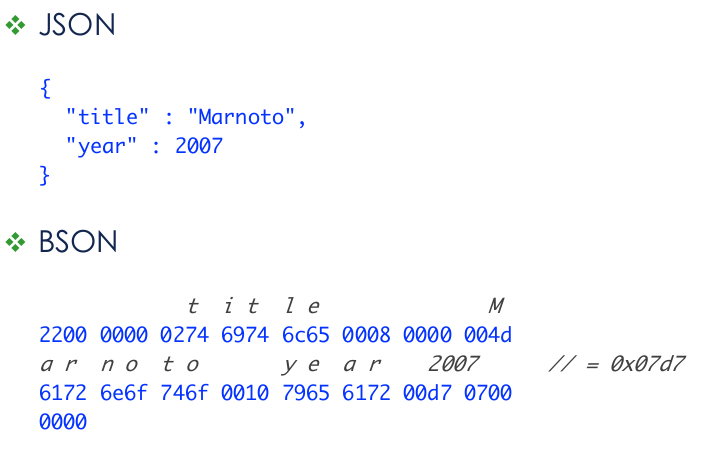
\includegraphics[scale=0.3]{57}
\end{center}

\pagebreak

\subsubsection*{Estrutura do Documento}

\begin{flushleft}
  \textbf{Documento:} Serialização de um objeto JSON ou array;

  O objeto JSON é serializado diretamente, e o array JSON é primeiro transformado
  num objeto JSON ([1, 2, 3] $\rightarrow$ \{"0": 1, "1": 2, "2": 3\});
\end{flushleft}

\begin{center}
  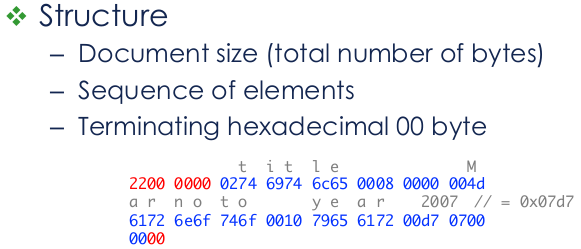
\includegraphics[scale=0.3]{58}
\end{center}

\begin{flushleft}
  \textbf{Elemento:} Serialização de uma propriedade JSON;
\end{flushleft}

\begin{center}
  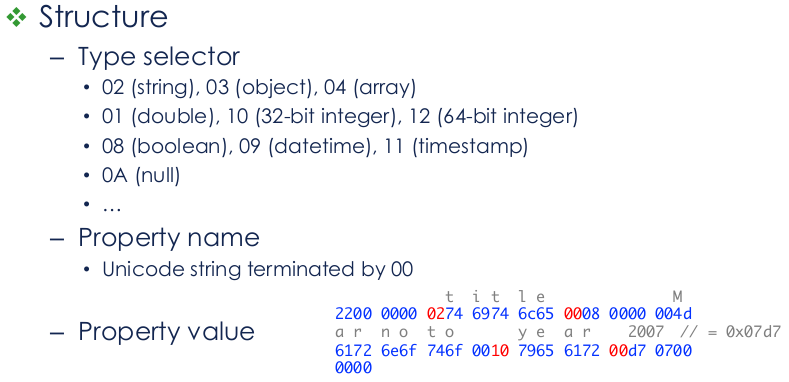
\includegraphics[scale=0.3]{59}
\end{center}

\subsubsection{RDF (Resource Description Framework)}

RDF é baseado no conceito em que todos os \textbf{recursos} podem ter diferentes \textbf{propriedades}
que têm \textbf{valores}.

\begin{flushleft}
  \textbf{Recursos:} Qualquer real-world entity
\end{flushleft}

\begin{center}
  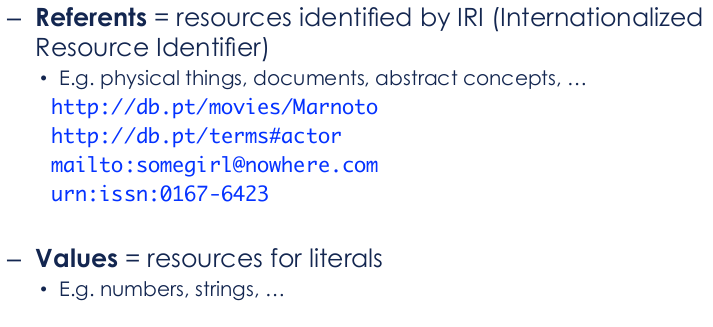
\includegraphics[scale=0.3]{60}
\end{center}

\pagebreak

\subsubsection*{Statements}

\begin{center}
  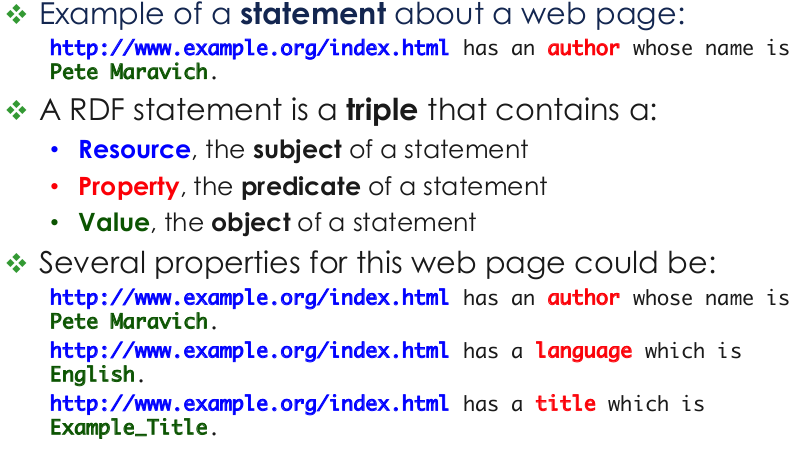
\includegraphics[scale=0.25]{61}
\end{center}

\subsubsection*{RDF Triple}

\begin{center}
  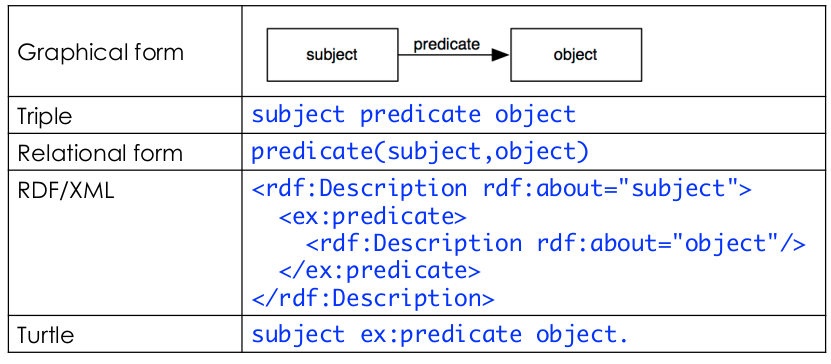
\includegraphics[scale=0.25]{62}
\end{center}

\subsubsection*{RDF Example}

\begin{center}
  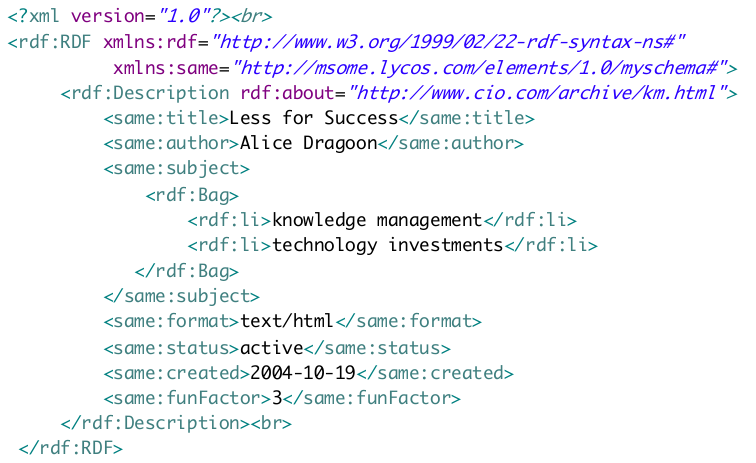
\includegraphics[scale=0.25]{63}
\end{center}

\subsection{Serialization approaches}

\begin{flushleft}
  \begin{itemize}
    \item RDF/XML notation (XML syntax para RDF);
    \item Turtle notation (Terse RDF Triple Language);
    \item N-Triples notation;
    \item JSON-LD notation (JSON-based serialization for Linked Data);
  \end{itemize}
\end{flushleft}

\pagebreak

\subsubsection{Turtle Notation}

Formato de texto compacto, várias abreviações para padrões de usage comuns.

\subsubsection*{Exemplo}

\begin{center}
  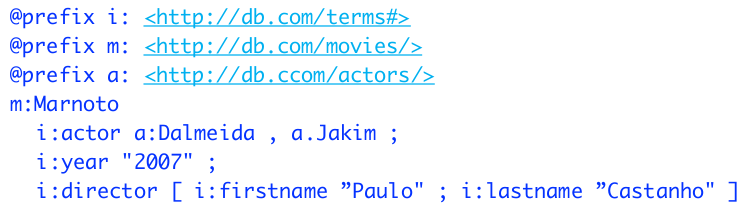
\includegraphics[scale=0.25]{64}
\end{center}

\subsection{Protocol Buffers}

Biblioteca de encoding \textbf{binário} que requer um \textbf{schema}
para os dados que estão encoded.

Mecanismo extensível para serializar dados estruturados. Usado em protocolos de
comunicação, data storage,\dots

Criado (e bastante usado) pela Google (maioritariamente para comunicação server-side).

Caracteristicas de desenho: \textbf{Fast}, \textbf{Small}, \textbf{Simple}.

File extension: *.proto

\begin{center}
  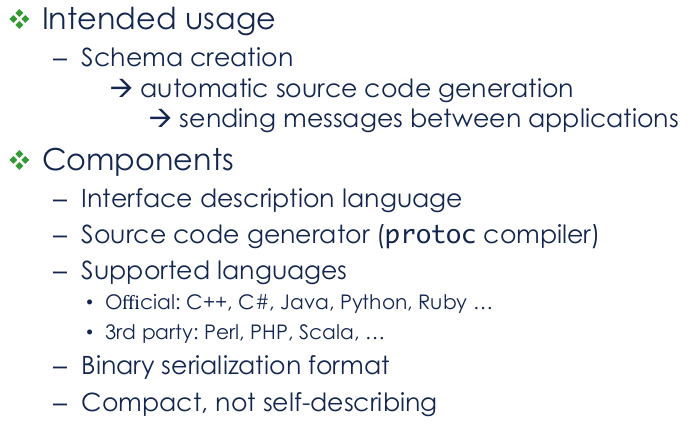
\includegraphics[scale=0.3]{65}
\end{center}

\subsubsection*{Schema: encoding examples}

\begin{center}
  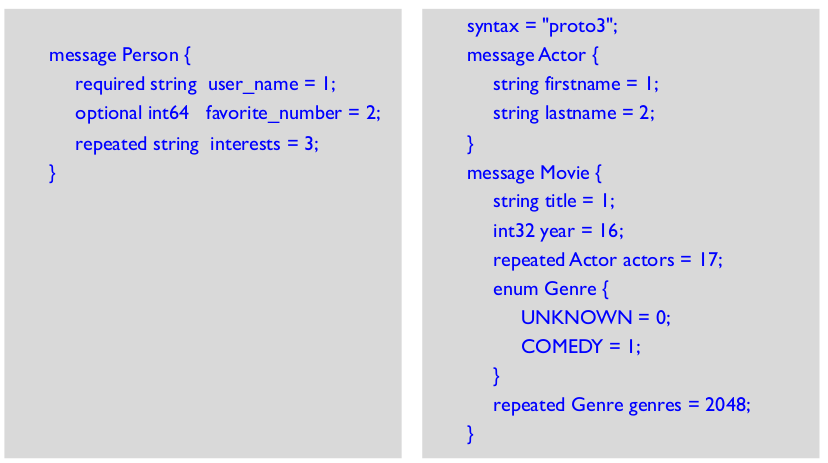
\includegraphics[scale=0.3]{66}
\end{center}

\pagebreak

\subsubsection*{Example: ProtoBuf to Java}

\begin{center}
  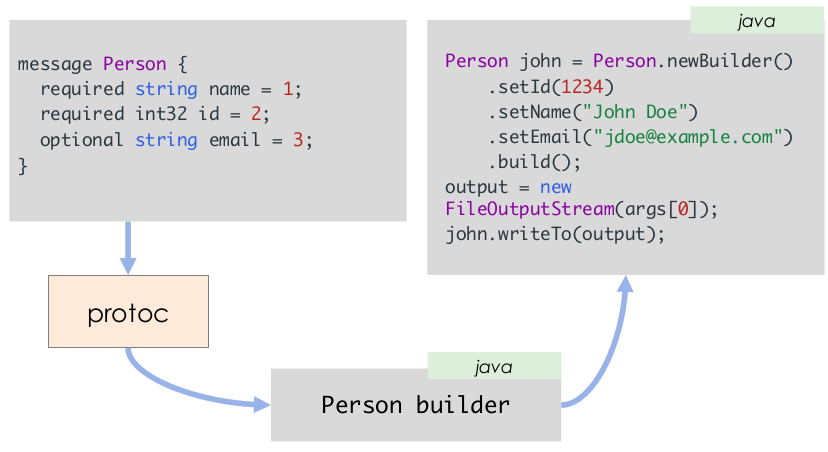
\includegraphics[scale=0.3]{67}
\end{center}

\pagebreak
\section{NoSQL Databases - Column Databases}

A ideia geral é que vamos \textbf{armazenar e processar dados por coluna} (column) em vez de por linha
(row). Geralmente tem origem em queries agregadores de dados, que permitem gerar
dados suscetíveis de serem analisados para fins \textbf{estatísticos} ou para \textbf{business intelligence}.

Visa então os \uline{serviços acima da utilização do armazenamento}, permitindo \textbf{processamento paralelo}
e consequentemente a construção de \textbf{aplicações de alto desempenho}.

A falta de normalização faz com que os dados sejam esparsos e que hajam bastantes campos
nulos. É descrita como: “sparse, distributed, persistent
multidimensional sorted map”.

\begin{center}
  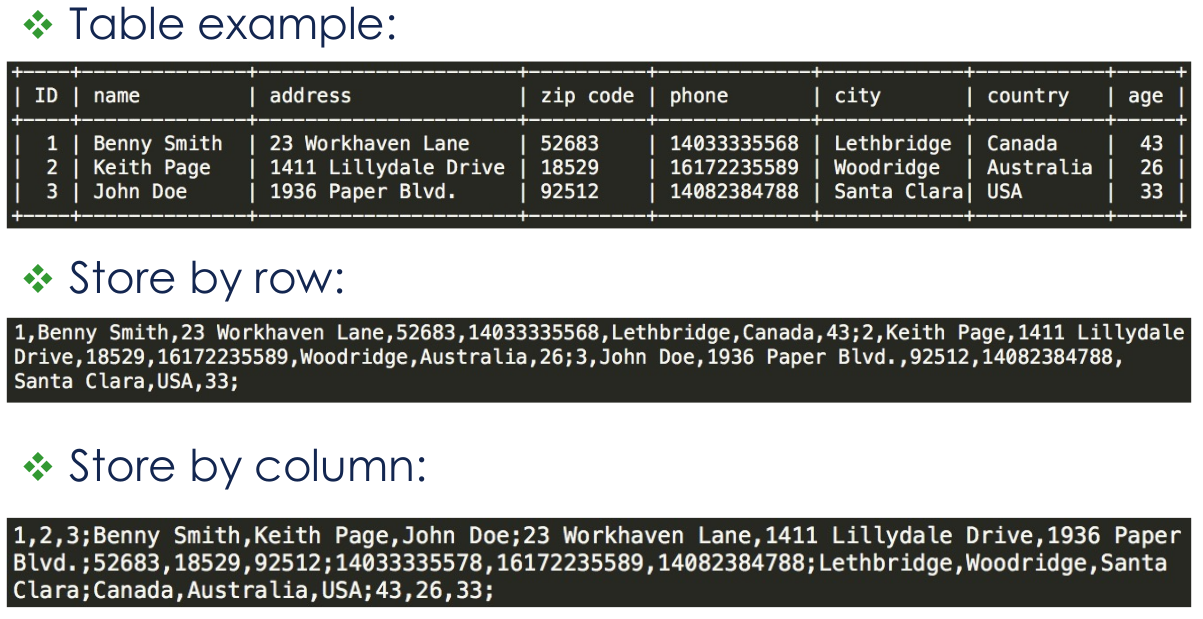
\includegraphics[scale=0.3]{10}
  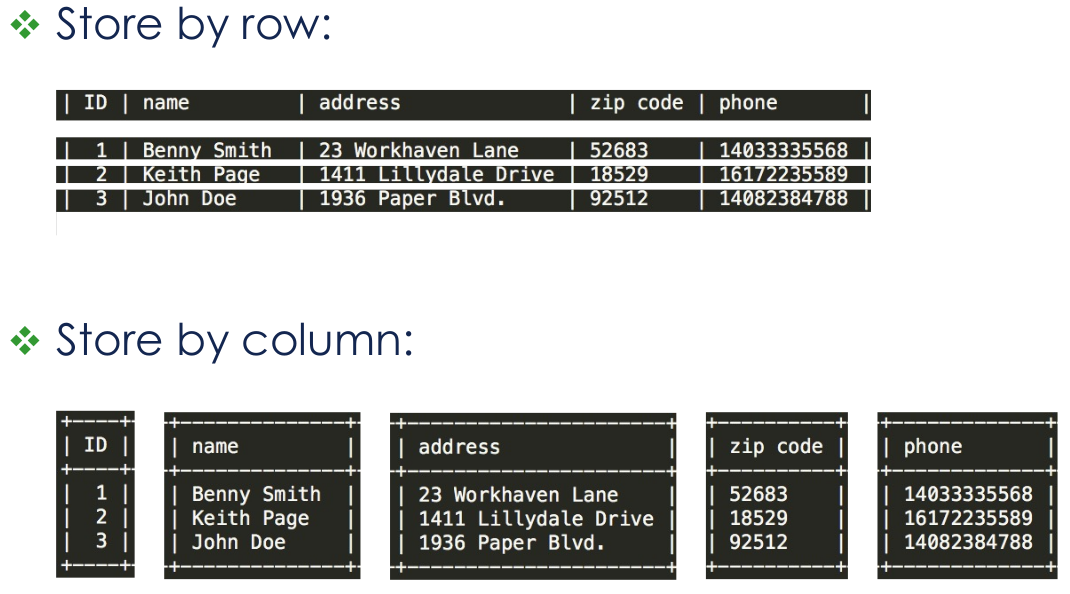
\includegraphics[scale=0.3]{11}
\end{center}

\pagebreak

\subsection{Vantagens}
É vantajoso em cenários em que são feitos \textbf{queries com poucas colunas sobre
grandes volumes de dados}. Destaca-se ainda a maior \textbf{facilidade de compressão} por colunas,
uma vez que estes dados neste domínio tendem a estar mais relacionados.

\subsubsection{Explicado}
Torna algumas queries mesmo muito rápidas:
\begin{itemize}
  \item Aggregation queries;
  \item Funções sobre fields (ex: average salary);
\end{itemize}
Melhor compressão de dados:
\begin{itemize}
  \item Ao correr o algoritmo em cada coluna (dados similares);
  \item Mais notável quando começamos a ter datasets grandes;
\end{itemize}

\subsection{Desvantagens}
Possui algumas desvantagens, como o \textbf{carregamento incremental de dados}, o uso de \textbf{OLTP}
(OnLine Transaction Processing), ou a realização de \textbf{queries a linhas} (dados individuais).

\subsubsection{Explicado}

Aggregation é bom, mas algumas aplicações precisam de ser capazes de mostrar dados para
cada \uline{individual record}. BDs colunares são geralmente não muito boas para esses tipos de queries.
Escrever novos dados pode demorar tempo, inserir um novo record numa row oriented database é uma simples
write operation. Fazer update de muitos values numa column db pode demorar muito tempo.

\vspace{2mm}

O \textbf{carregamento incremental} de dados caracteriza-se por atualizações constantes. É uma desvantagem porque a cada
inserção têm de se editar todos os ficheiros de todas as colunas, pelo que este processo geralmente é realizado
periodicamente e para grandes volumes de dados em simultâneo.

\vspace{2mm}

Contrariamente às bases de dados relacionais, são \textbf{orientadas aos serviços}
e não aos dados.

\vspace{2mm}

Nasceu com o projeto \textbf{Bigtable} da Google, que serviu de inspiração
aos restantes SGBD's colunares. Foi criado em resposta ao problema de greração
de índices para o seu motor de busca, que levava demasiado tempo.
Atualmente é utilizado também no Gmail e Google Maps.

\pagebreak

\subsection{Modelo de Dados}

\begin{flushleft}
  \textbf{Familia de colunas (tabela)} - Uma tabela é uma coleção de linhas semelhantes
  (não necessariamente idênticas).

  \textbf{Linha} - Uma linha é um conjunto de colunas (deve abranger um grupo de dados
  que é acessado em conjunto).
  Associado com uma chave de linha (row key) única.

  \textbf{Coluna} - Uma coluna consiste num nome de coluna (column name)
  e um valor de coluna (column value), possivelmente outros records de metadados.
  Valores escalares, mas também sets, listas e mapas.
\end{flushleft}

\subsection{Casos de Uso}

As bases de dados orientadas a colunas são utilizadas para o armazenamento de
dados estrutrados com um esquema similar, como log de eventos, sistemas de
gestão de conteúdo, blogs, \dots

Processamento de dados em batch via MapReduce.

\vspace{2mm}

Não é recomendado a utilização deste tipo de bases de dados quando
\textbf{transições ACID} (atomicidade, consistência, isolamento, durabilidade) são necessárias,
quando é necessário usar \textbf{queries complexas} como joins, nem \textbf{prototipagem} (o design da BD pode mudar), uma vez que a
sua orientação ao serviço, a torna altamente dependente dos seus requisitos.

\subsection{Tecnologias Representativas}

\begin{center}
  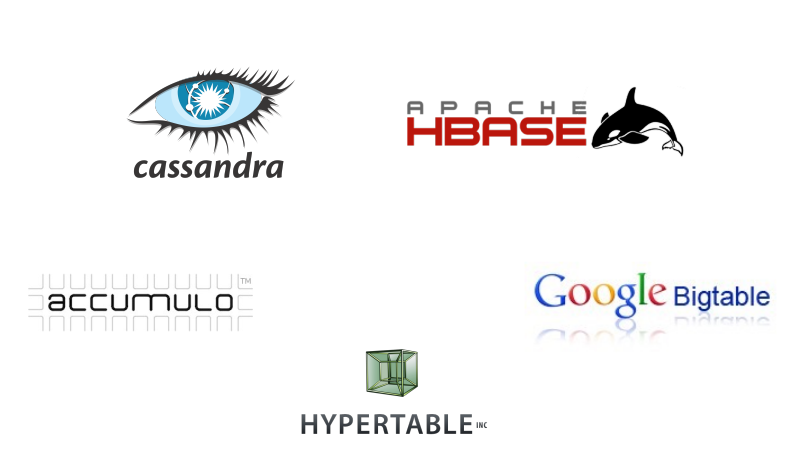
\includegraphics[scale=0.3]{12}
\end{center}

\textbf{Bigtable} é a inspiração para as datastores orientadas a colunas.
Bases de daods influenciadas pela Bigtable:
\begin{itemize}
  \item \textbf{HBase}
  \item \textbf{HyperTable}
\end{itemize}

\textbf{Cassandra} é uma extensão da Bigtable com aspetos do Dynamo da Amazon.

\pagebreak

\subsection{Apache Cassandra}

\subsubsection{Introdução}

É uma Cross Plataform, \textbf{open-source} Column Database, cujas features incluem
\textbf{alta disponibilidade}, \textbf{escalabilidade linear},
\textbf{fragmentação}, \textbf{replicação P2P configuravél},
\textbf{consistência tunable} e \textbf{suporte para MapReduce}.

Atualmente é o sistema de bases de dados orientado a colunas mais utilizado.
Foi inicialmente desenvolvido pelo Facebook (2008) mas atualmente está sob gestão da
fundação para o software Apache.

É ainda de destacar o alto desempenho na escrita, sem prejudicar a eficiência das leituras.
Por exemplo: Para dados com uma dimensão superior a 50GB, as escritas e leituras levariam cerca de 300ms. A Cassandra oferece
leituras a 0,12ms e escritas a 0,15ms.

\subsubsection{Motivação}
\begin{itemize}
  \item High availability;
  \item High write throughput, sem sacrificar read efficiency;
  \item Fault tolerance;
  \item High and incremental scalability;
  \item Reliablility at massive scale;
\end{itemize}

\subsubsection{Topologia do Sistema}

\begin{center}
  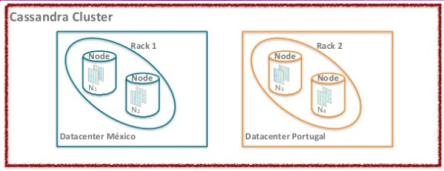
\includegraphics[scale=0.3]{13}
\end{center}

\begin{flushleft}
  \textbf{Node} - É a unidade base destes sistemas, são máquinas
  onde a Cassandra está em execução.

  \vspace{2mm}

  \textbf{Data Center} - Os nós são agrupados em data centers.
  Conjunto de nós relacionados entre si, que fazem \uline{replicação dos dados}
  de forma a garantir a \textbf{tolerância a falhas}.

  \vspace{2mm}

  \textbf{Cluster} - Conjunto de data centers sobre os quais são escritos
  os mesmo dados.
\end{flushleft}

\pagebreak

\subsubsection{Arquitetura do Sistema}

\begin{flushleft}
  \textbf{Cluster Membership} - Como é que os nodes são adicionados ou
  apagados de um cluster.

  \vspace{2mm}

  \textbf{Partitioning}
  \begin{itemize}
    \item Como é que os dados são particionados pelos nodes;
    \item Nodes são logicamente estruturados numa \textbf{Ring Topology};
    \item Hashed Values e Keys associados a Data Partitions são usadas para
    lhes dar assign a um node no ring.
  \end{itemize}

  \vspace{2mm}

  \textbf{Replication}
  \begin{itemize}
    \item Como é que os dados são duplicados pelos nós;
    \item Cada DataItem é replicado por N (replication factor) Nodes.
  \end{itemize}
\end{flushleft}

\subsubsection{Topologia do Sistema}

\begin{center}
  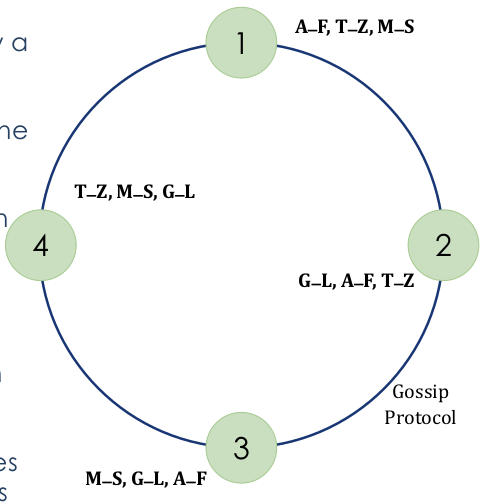
\includegraphics[scale=0.3]{14}
\end{center}

\begin{itemize}
  \item Cluster Data é gerida por um Ring of Nodes;
  \item Cada Node tem parte da BD;
  \item Rows são distribuidas baseadas na primary key;
  \item Rows são distribuidas baseadas na primary key (Row Lookups são rápidos);
  \item Múltiplos nodes tem os mesmos dados, para garantir availability e durability;
  \item Não há nenhum master node - Todos os nodes podem realizar todas as operações;
\end{itemize}

\pagebreak

\subsubsection{Modelo de dados}
\subsubsection*{Keyspaces $>$ Tables $>$ Rows $>$ Columns}

\begin{flushleft}
  \textbf{Keyspace:}
  \begin{itemize}
    \item É um \textbf{namespace} que define data replication nos nodes;
    \item Um cluster contém \textbf{um keyspace por node};
  \end{itemize}

  \vspace{2mm}

  \textbf{Table (Column Family):}
  \begin{itemize}
    \item Coleção de rows (parecidas);
    \item Multi-Dimensional Map indexado por chave (row key);
    \item Tables Schema tem de ser especificado mas pode ser modificado;
    \item 2 tipos: Simple ou Super (nested Column Families);
  \end{itemize}

  \vspace{2mm}
  
  \textbf{Row:}
  \begin{itemize}
    \item Coleção de colunas;
    \item Rows numa table não precisam de ter as mesmas colunas
    \item Cada Row É \textbf{uniquely identified} por uma \textbf{primary key};
  \end{itemize}

  \vspace{2mm}

  \textbf{Column:}
  \begin{itemize}
    \item Name-Value Pair + Dados Adicionais;
  \end{itemize}
\end{flushleft}

\begin{figure}[!h]
  \centering
  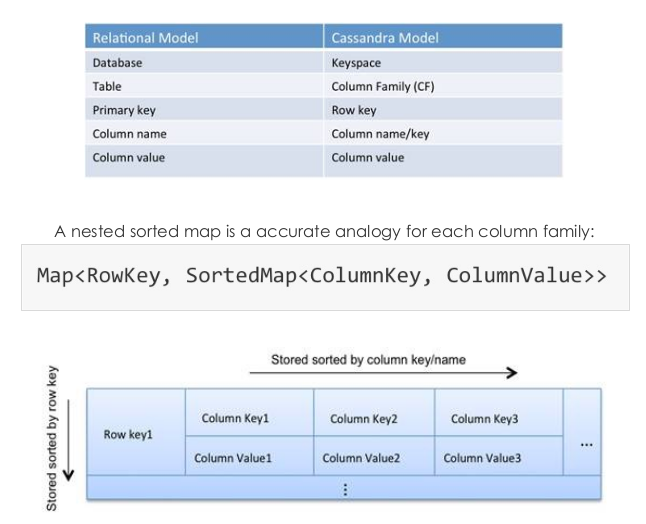
\includegraphics[scale=0.3]{15}
  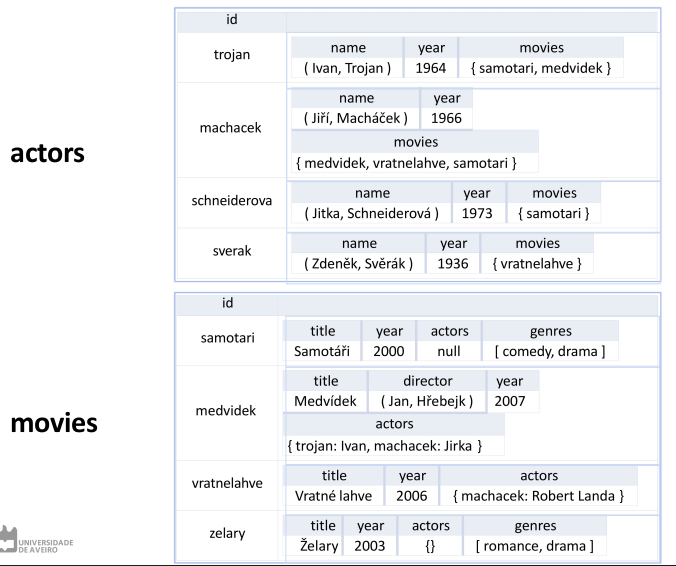
\includegraphics[scale=0.3]{16}
  \caption{Exemplo de um Data Model}
\end{figure}

\pagebreak

\subsubsection{Cassandra vs Relational Example}

\begin{figure}[!h]
  \centering
  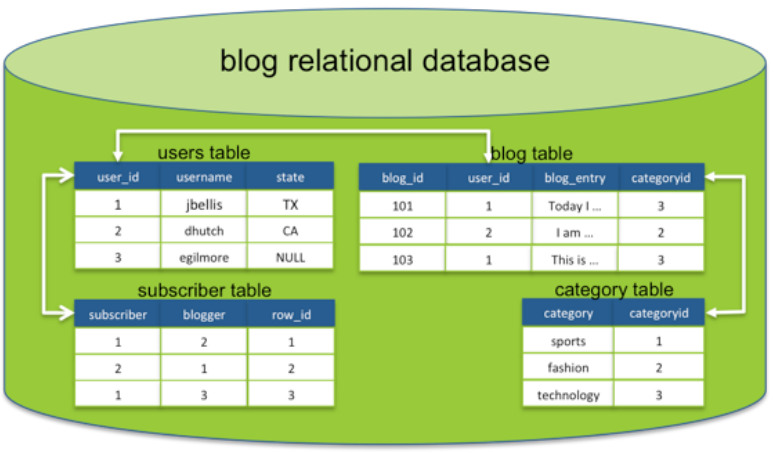
\includegraphics[scale=0.25]{17}
  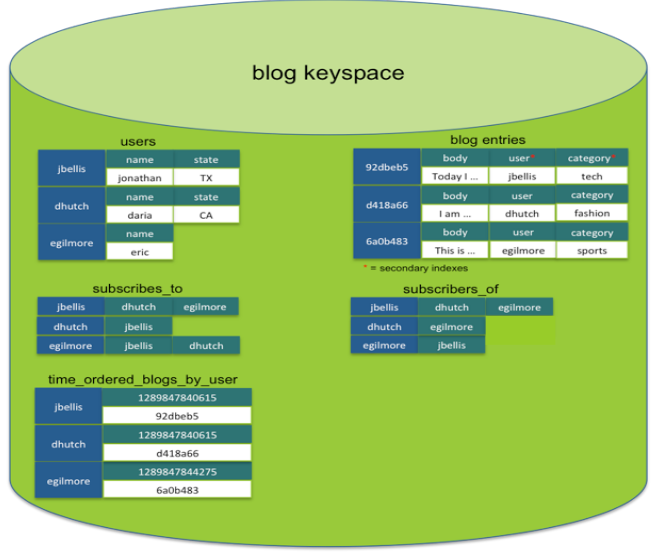
\includegraphics[scale=0.25]{18}
\end{figure}

\subsubsection{Column Values}
\begin{flushleft}
  Os value types aceites pelas colunas são:
  \begin{itemize}
    \item \textbf{Empty Value}
    \begin{itemize}
      \item Null
    \end{itemize}
    \item \textbf{Atomic Value}
    \begin{itemize}
      \item \textbf{Native Data Types} (Text, Integers, Dates, \dots)
      \item \textbf{Tuples} (Tuplo de fields anonimos, cada um com o seu Type
      (podendo cada membro do tuplo ter um type diferente))
      \item \textbf{User Defined Types (UDT)} (Set de named fields para cada type)
    \end{itemize}
    \item \textbf{Collections}
    \begin{itemize}
      \item \textbf{Lists}, \textbf{Sets} e \textbf{Maps} (Nested Tuples, UDTs ou collections são
      permitidos mas apenas um Forzen Mode (elementos são serializados quando
      são guardados))
    \end{itemize}
  \end{itemize}
\end{flushleft}

\subsubsection{Data Model - Dados adicionais}

Associados a cada coluna no caso dos atomic values ou qualquer element de uma
collection.

\begin{flushleft}
  \textbf{Time to Live (TTL):} Após um certo tempo (segundos) um dado value é automaticamente apagado;

  \vspace{2mm}

  \textbf{Timestamp:} Timestamp de quando a última modificação foi feita. Fornecido
  automaticamente ou manualmente;
\end{flushleft}

Ambos estes elementos podem ser queried mas não no caso de collections e dos seus
elementos.

\pagebreak

\subsubsection{Cassandra API}

\begin{flushleft}
  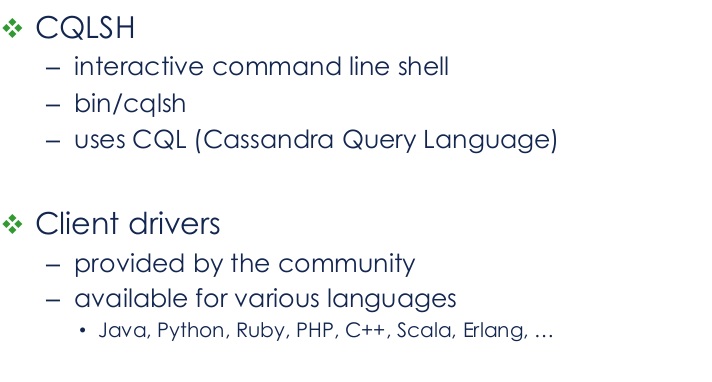
\includegraphics[scale=0.3]{19}
\end{flushleft}

\subsection{Cassandra Query Language (CQL)}

Declarative query language inspired by SQL.

\begin{center}
  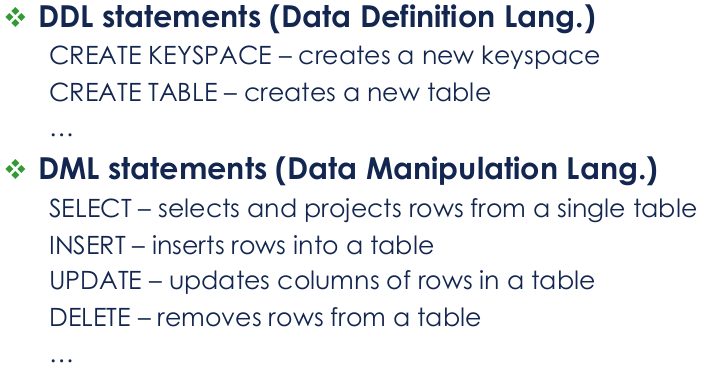
\includegraphics[scale=0.3]{20}
\end{center}

\subsubsection{Keyspace}

\begin{figure}[!h]
  \centering
  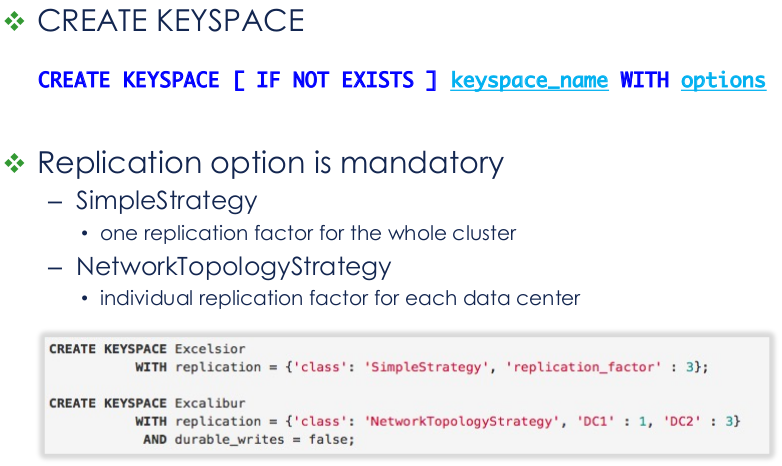
\includegraphics[scale=0.25]{21}
  \includegraphics[scale=0.25]{22}
\end{figure}

\pagebreak

\subsubsection{Table - Create Statement}

\begin{center}
  \includegraphics[scale=0.25]{23}
\end{center}

\subsubsection{Table - Primary Key}

\begin{flushleft}
  Primary key has 2 parts:

  \textbf{Compulsory Partition Key:} 
  \begin{itemize}
    \item Uma ou mais colunas;
    \item Descreve como é que as table rows são distribuidas pelas partitions
  \end{itemize}

  \textbf{Optional Clustering Key (ou Columns):}
  \begin{itemize}
    \item Define a Clustering Order, isto é, como é que as tables estão localmente
    guardadas dentro de uma partição;
  \end{itemize}

  \begin{center}
    \includegraphics[scale=0.3]{24}
  \end{center}
\end{flushleft}

\subsubsection{Key Roles}

\begin{flushleft}
  \textbf{Partition Key:} Responsável por da Distribution (partitioning)
  pelos nodes da BD. Pode ter multiplas colunas.
  
  \vspace{2mm}

  \textbf{Clustering Key:} Responsável oir Data Sorting dentro de uma partition.
  Pode ter multiplas colunas.

  \vspace{2mm}

  \textbf{Primary Key:} Equivalente a uma Partition Key num Single-Field-Key Table;

  \vspace{2mm}

  \textbf{Composite Key:} Multiple-Column Key

  \begin{figure}[!h]
    \centering
    \includegraphics[scale=0.3]{25}
    \caption{Exemplo de uma Composite Key}
  \end{figure}
\end{flushleft}

\pagebreak

\subsubsection{Table - Other Statements}

\begin{center}
  \includegraphics[scale=0.3]{26}
\end{center}

\subsubsection{Select Statement}

\begin{center}
  \includegraphics[scale=0.3]{27}
\end{center}

\subsubsection{Select - FROM Clause}

\begin{flushleft}
  Define uma \textbf{única tabela} para a query:
  \begin{itemize}
    \item do keyspace atual/especificado;
    \item \uline{dar join a outras tabelas não é possível};
  \end{itemize}

  \pagebreak

  Suporta:
  \begin{itemize}
    \item \textbf{distinct} para eliminar rows duplicadas;
    \item (user-defined) \textbf{aggregate functions}
    \item \textbf{*} para selecionar todas as colunas;
    \item \textbf{AS} para atribuit um alias a uma coluna;
    \item WRITETIME (timestamp) e TTL (time to live) para selecionar os valores
    de timestamp e ttl de uma coluna (não pode ser usado na clausula WHERE);
  \end{itemize}

  \begin{center}
    \includegraphics[scale=0.3]{28}
  \end{center}
\end{flushleft}

\subsubsection{Select - WHERE Clause}

\begin{flushleft}
  Sintaxe parecidas entre CQL e SQL.

  As diferenças aparecem devido ao facto da Cassandra estar a lidar com dados
  distribuidos, logo temos de procurar prevenir queries ineficientes
  \begin{itemize}
    \item Rows estão espalhadas pelo cluster baseado na Hash das suas partition keys;
    \item Clustering keys são usadas para fazer cluster dos dados de uma partição
    permitindo um retrieval muito eficiente das rows;
  \end{itemize}

  \vspace{2mm}

  \textbf{Nota:} Partition Key, Clustering e normal columns supostam diferentes
  sets de restrições dentro da clausula WHERE.

  \vspace{2mm}

  \textbf{Partition Key Columns:}
  \begin{itemize}
    \item Suportam \textbf{=} e \textbf{IN};
    \item Todas as primary keys columns tem de ser usadas (restricted),
    a não ser que tenhasmos secondary indexes;
    \item Todas as colunas são precisas para computar a hash que vai permirie localizar
    os nós que contenham os dados partição;
  \end{itemize}

  \vspace{2mm}

  \textbf{Clustering Key:}
  \begin{itemize}
    \item Suportam \textbf{=, $<$, $>$, $<$=, $>$=};
    \item \textbf{IN} retorna verdadeiro se o valor for um dos enumerados;
    \item \textbf{CONTAINS*} e \textbf{CONTAINS KEY}:
    \begin{itemize}
      \item Retornam True se a coleção contiver o dado elemento;
      \item Quando o query estiver a usar um secondary index;
      \item Usado em collections* (lists, sets, maps) / maps**; 
    \end{itemize}
  \end{itemize}
\end{flushleft}

\pagebreak

\subsubsection*{Examples:}

\begin{center}
  \includegraphics[scale=0.35]{29}
\end{center}

\begin{center}
  \includegraphics[scale=0.35]{30}
\end{center}

\begin{center}
  \includegraphics[scale=0.3]{31}
\end{center}

\pagebreak

\subsubsection{Select - GROUP BY, ORDER BY \& LIMIT}

\begin{flushleft}
  \textbf{GROUP BY} clause:
  \begin{itemize}
    \item Agrupar Rows de uma Table de acordo com certas colunas;
    \item \textbf{Apenas grouping induzidos por primary key columns são permitidos};
    \item Quando non-grouping columns são selecionadas sem uma aggregate function,
    o primeiro value encontrado é sempre retornado;
  \end{itemize}

  \vspace{2mm}

  \textbf{ORDER BY} clause:
  \begin{itemize}
    \item Define a ordem (ASC ou DESC) das rows retornadas;
    \item \textbf{Partition Key tem de ser restricted com = ou IN};
    \item \textbf{APENAS} orderings induzidos por \textbf{CLUSTERING COLUMNS} são permitidos;
  \end{itemize}

  \vspace{2mm}

  \textbf{LIMIT} clause:
  \begin{itemize}
    \item Limita o número de rows retornadas numa query result;
  \end{itemize}

  \begin{center}
    \includegraphics[scale=0.3]{32}
  \end{center}
\end{flushleft}

\subsubsection{Select - User Defined Functions}

\begin{center}
  \includegraphics[scale=0.3]{33}
\end{center}

\pagebreak

\subsubsection{Select - Aggregates}

\begin{center}
  \includegraphics[scale=0.3]{34}
\end{center}

\subsubsection{Select - ALLOW FILTERING}

\begin{center}
  \includegraphics[scale=0.3]{35}
\end{center}

\pagebreak

\subsubsection{Insert Statement}

\begin{flushleft}
  Insere uma nova row numa dada table:
  \begin{itemize}
    \item Se a Primary Key existir, a row é atualizada;
    \item Existe a \textbf{condição IF NOT EXISTS} para apenas inserir caso uma row não exista;
  \end{itemize}

  Escreve uma ou mais colunas para uma dada row.
  Pelo menos as Primeary Key Columns têm de ser especificadas.

  \begin{center}
    \includegraphics[scale=0.3]{36}
  \end{center}
\end{flushleft}

\subsubsection{Update Statement}

\begin{flushleft}
  Atualiza rows existentes dentro de uma dada table:
  \begin{itemize}
    \item Se a row com a dada primary key não existir, é inserida; 
  \end{itemize}

  Todas as Primary Key Columns têm de ser especificadas na clausula WHERE.

  \begin{figure}[!h]
    \centering
    \includegraphics[scale=0.3]{37}
    \includegraphics[scale=0.3]{38}
  \end{figure}
\end{flushleft}

\pagebreak

\subsubsection{Parametros Insert \& Update}

\begin{center}
  \includegraphics[scale=0.25]{39}
\end{center}

\subsubsection{Delete Statement}

\begin{flushleft}
  Remove existing rows/columns/collection elements de uma dada tabela.

  A clausula \textbf{WHERE} é usada para especificar qual a row que queremos deleted.

  Múltiplas Rows podem ser apagadas com uma única query usando o operador \textbf{IN}.

  Um range de rows pode ser apagado usando um inequality operator ($<$, $>$, $<=$, $>=$).

  \begin{center}
    \includegraphics[scale=0.3]{40}
  \end{center}
\end{flushleft}

\end{document}
